\documentclass[AutoFakeBold,AutoFakeSlant]{beamer}
\usepackage{ctex}
\usepackage{hyperref}
\bibliographystyle{plain}
\usepackage[defaultsans]{droidsans}
\usepackage{fontspec}
\usepackage{newtxmath}
\usepackage{latexsym,amsmath,xcolor,multicol,booktabs,calligra,tcolorbox}
\usepackage{graphicx,tabularx,multirow,makecell}

% 主题设置（使用干净简洁的Madrid主题）
\usetheme{Madrid}
\usecolortheme{default}
\setbeamertemplate{navigation symbols}{}
\setbeamertemplate{footline}[frame number]

% 定义新命令
\newcommand{\ba}{\backslash}
\newcommand{\Q}{\mathbb{Q}}
\newcommand{\C}{\mathbb{C}}
\newcommand{\R}{\mathbb{R}}
\newcommand{\N}{\mathbb{N}}
\newcommand{\Z}{\mathbb{Z}}
\newcommand{\F}{\mathbb{F}}
\newcommand{\rank}{\text{rank}}

% 列表设置
\usepackage{listings}
\lstset{
	columns = fixed,
	basewidth = {0.5em},
	breaklines = true,
	backgroundcolor = \color{white},
	keywordstyle = \color{blue},
	numberstyle = \footnotesize\color{darkgray},
	commentstyle = \ttfamily\color{violet},
	basicstyle = \small\ttfamily,
	stringstyle = \ttfamily\color{green!40!black},
	showstringspaces = false,
}

% 作者信息
\author{李禹江 张博涵 蒋兴宇}
\title{中美欧数据隐私法规对比研究}
\subtitle{基于PIPL、GDPR、CCPA的六维分析}
\institute{我的刀盾队} 
\date{\today}

\begin{document}
\kaishu

\begin{frame}
    \titlepage
\end{frame}

\begin{frame}
	\frametitle{目录}
	\tableofcontents
\end{frame}

\section{研究方法}
\begin{frame}
	\frametitle{研究方法}
	\begin{itemize}
		\item \textbf{文献研究法}：系统梳理三部法律原文及修订案、官方指南、学术文献。
		\item \textbf{比较分析法}：从六个核心维度横向对比三部法律的异同。
		\item \textbf{量化评估法}：构建"作用范围"与"严格程度"两个指标，以星级进行可视化度量。
	\end{itemize}
\end{frame}

\section{研究目的}
\begin{frame}
	\frametitle{研究目的}
	\begin{itemize}
		\item 基于法律文件了解各法域中数据隐私保护的执行依据。
		\item 为隐私检测软件开发提供精确、可落地的合规规则库。
		\item 明确各法域在跨境流动、监管处罚、主体权利等方面的核心要求与差异。
	\end{itemize}
\end{frame}

\section{研究内容}
\begin{frame}
	\frametitle{研究内容}
	从以下六个维度,共二十九个具体内容展开系统对比：
	\begin{enumerate}
		\item 基础概念与适用范围
		\item 处理的核心原则与合法性
		\item 数据主体的权利
		\item 处理者的义务与合规
		\item 数据的跨境流动
		\item 监管与法律责任
	\end{enumerate}
	每个维度均包含具体条款对比及作用范围/严格程度量化评级。
\end{frame}

\begin{frame}
	\frametitle{分类依据}
	作用范围：指该法律条款在地域、对象、数据类型等方面的覆盖广度。
	\begin{enumerate}
	\item 小：覆盖范围非常有限，存在大量豁免或仅适用于极少数情形。

	\item 中：覆盖范围中等，有明确限定但基本涵盖核心领域。

	\item 大：覆盖范围最广，长臂管辖、对象定义宽泛、数据活动全面。
	\end{itemize}
	严格程度：指该法律条款对企业的合规要求强度、处罚力度、权利保护水平。
	\begin{enumerate}
	\item 小：要求宽松，义务较少，处罚轻或无实质制裁。

	\item 中：有明确的义务和一定处罚，但留有较多灵活空间。

	\item 大：要求极为严格，处罚上限高，权利保护全面且难以豁免。
	\end{itemize}
	每个小点的星级由前述对比分析中的具体条款内容决定，确保评分有据可依。
\end{frame}

\section{研究结果}

\subsection{基础概念与适用范围}
\begin{frame}
	\frametitle{基础概念与适用范围}
	\scriptsize
	\begin{tabularx}{\textwidth}{X|X|X|X}
		\toprule
		\textbf{比较点} & \textbf{PIPL} & \textbf{GDPR} & \textbf{CCPA/CPRA} \\
		\midrule
		地域范围 & 境内+境外向境内提供服务/分析行为 & 境内+境外向欧盟主体提供商品/监控 & 在加州"开展业务"，商业行为全部在境外则不适用 \\
		规制对象 & 个人信息处理者 & 控制者、处理者 & 符合门槛的营利性企业、服务提供商等 \\
		数据活动 & 收集、存储、使用、加工、传输、提供、公开、删除等 & 收集、记录、组织、存储、修改、检索、披露、擦除等 & 重点规制"销售"和"共享" \\
		排除范围 & 个人/家庭事务、政府统计 & 非欧盟法律活动、外交/安全、个人/家庭、执法 & 受HIPAA、GLBA、FCRA规制的数据 \\
		个人信息定义 & 与已识别/可识别自然人有关的信息（不含匿名化） & 与已识别/可识别自然人相关的任何信息 & 识别/描述特定消费者或家庭的信息（排除政府公开记录） \\
		匿名化/去识别化 & 匿名化不属于个人信息；去标识化仍属个人信息 & 假名化仍属个人数据；彻底匿名化不适用 & 去识别化（不重识别）不属于个人信息 \\
		\bottomrule
	\end{tabularx}
\end{frame}

\begin{frame}
	\frametitle{基础概念与适用范围 - 星级对比}
	\centering
	\textbf{作用范围星级对比}
	\begin{figure}
		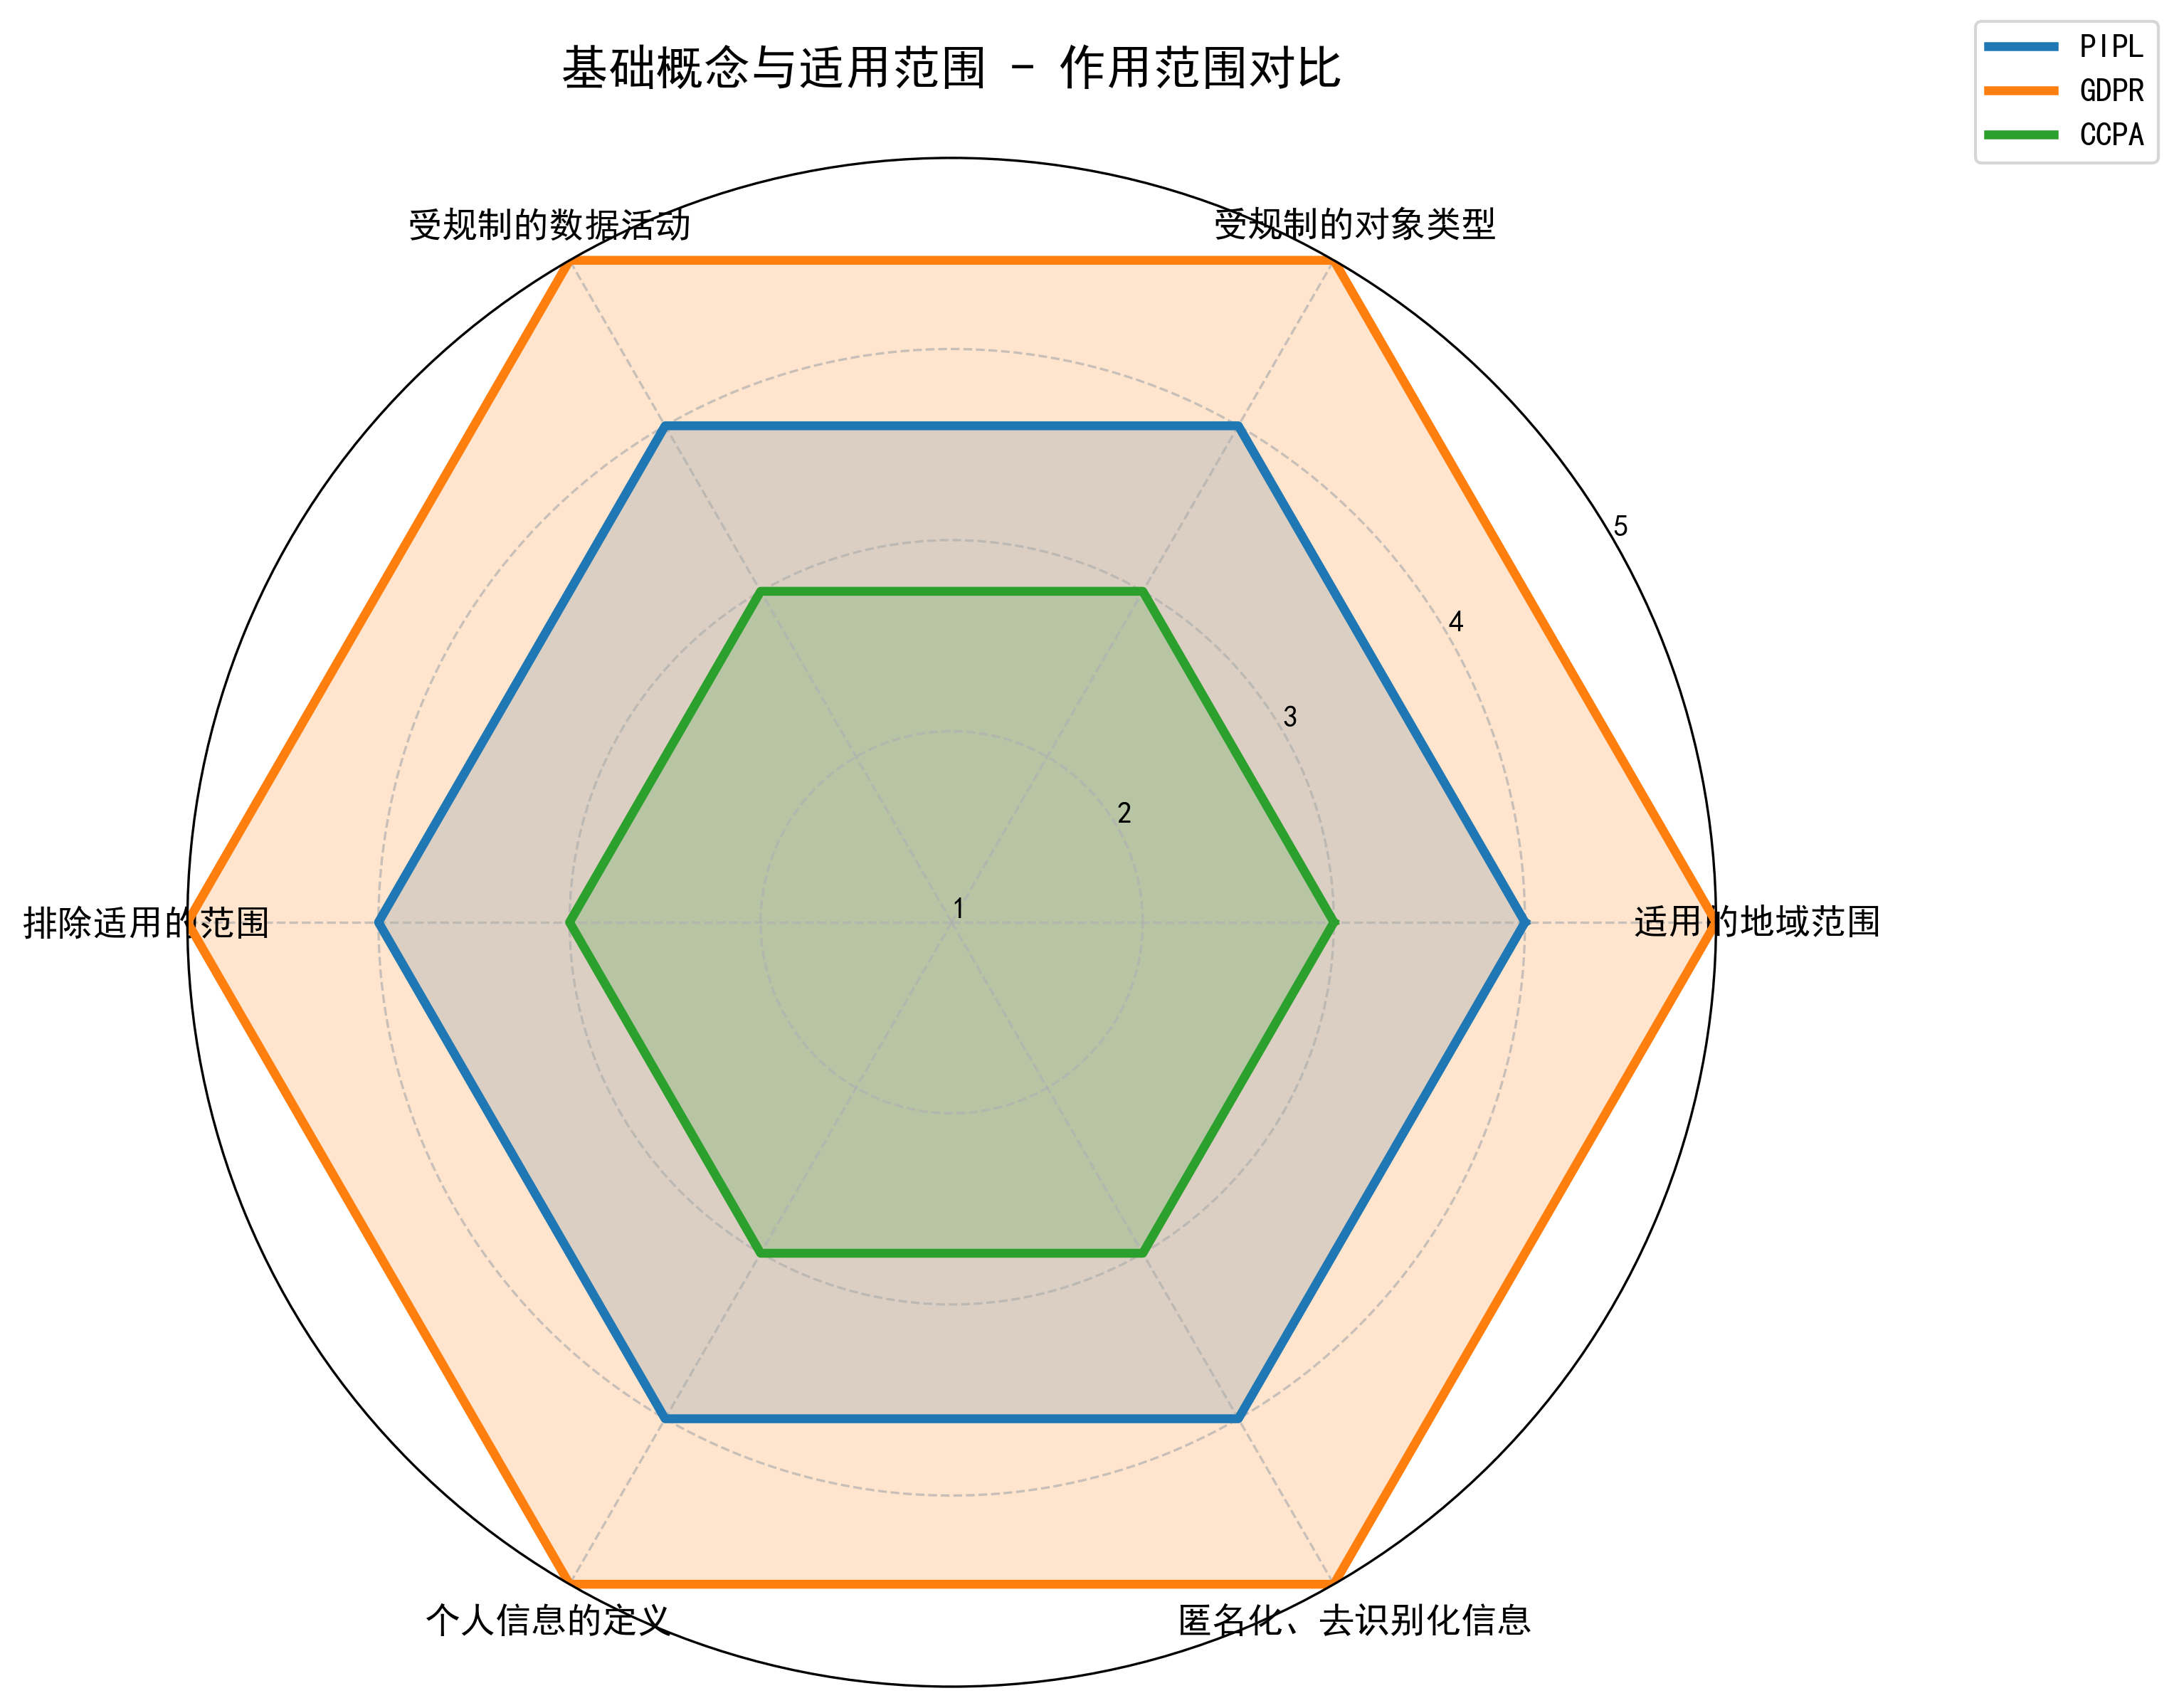
\includegraphics[width=0.8\textwidth]{pics/radar_基础概念与适用范围_scope.png}
	\end{figure}
\end{frame}

\begin{frame}
	\frametitle{基础概念与适用范围 - 星级对比}
	\centering
	\textbf{严格程度星级对比}
	\begin{figure}
		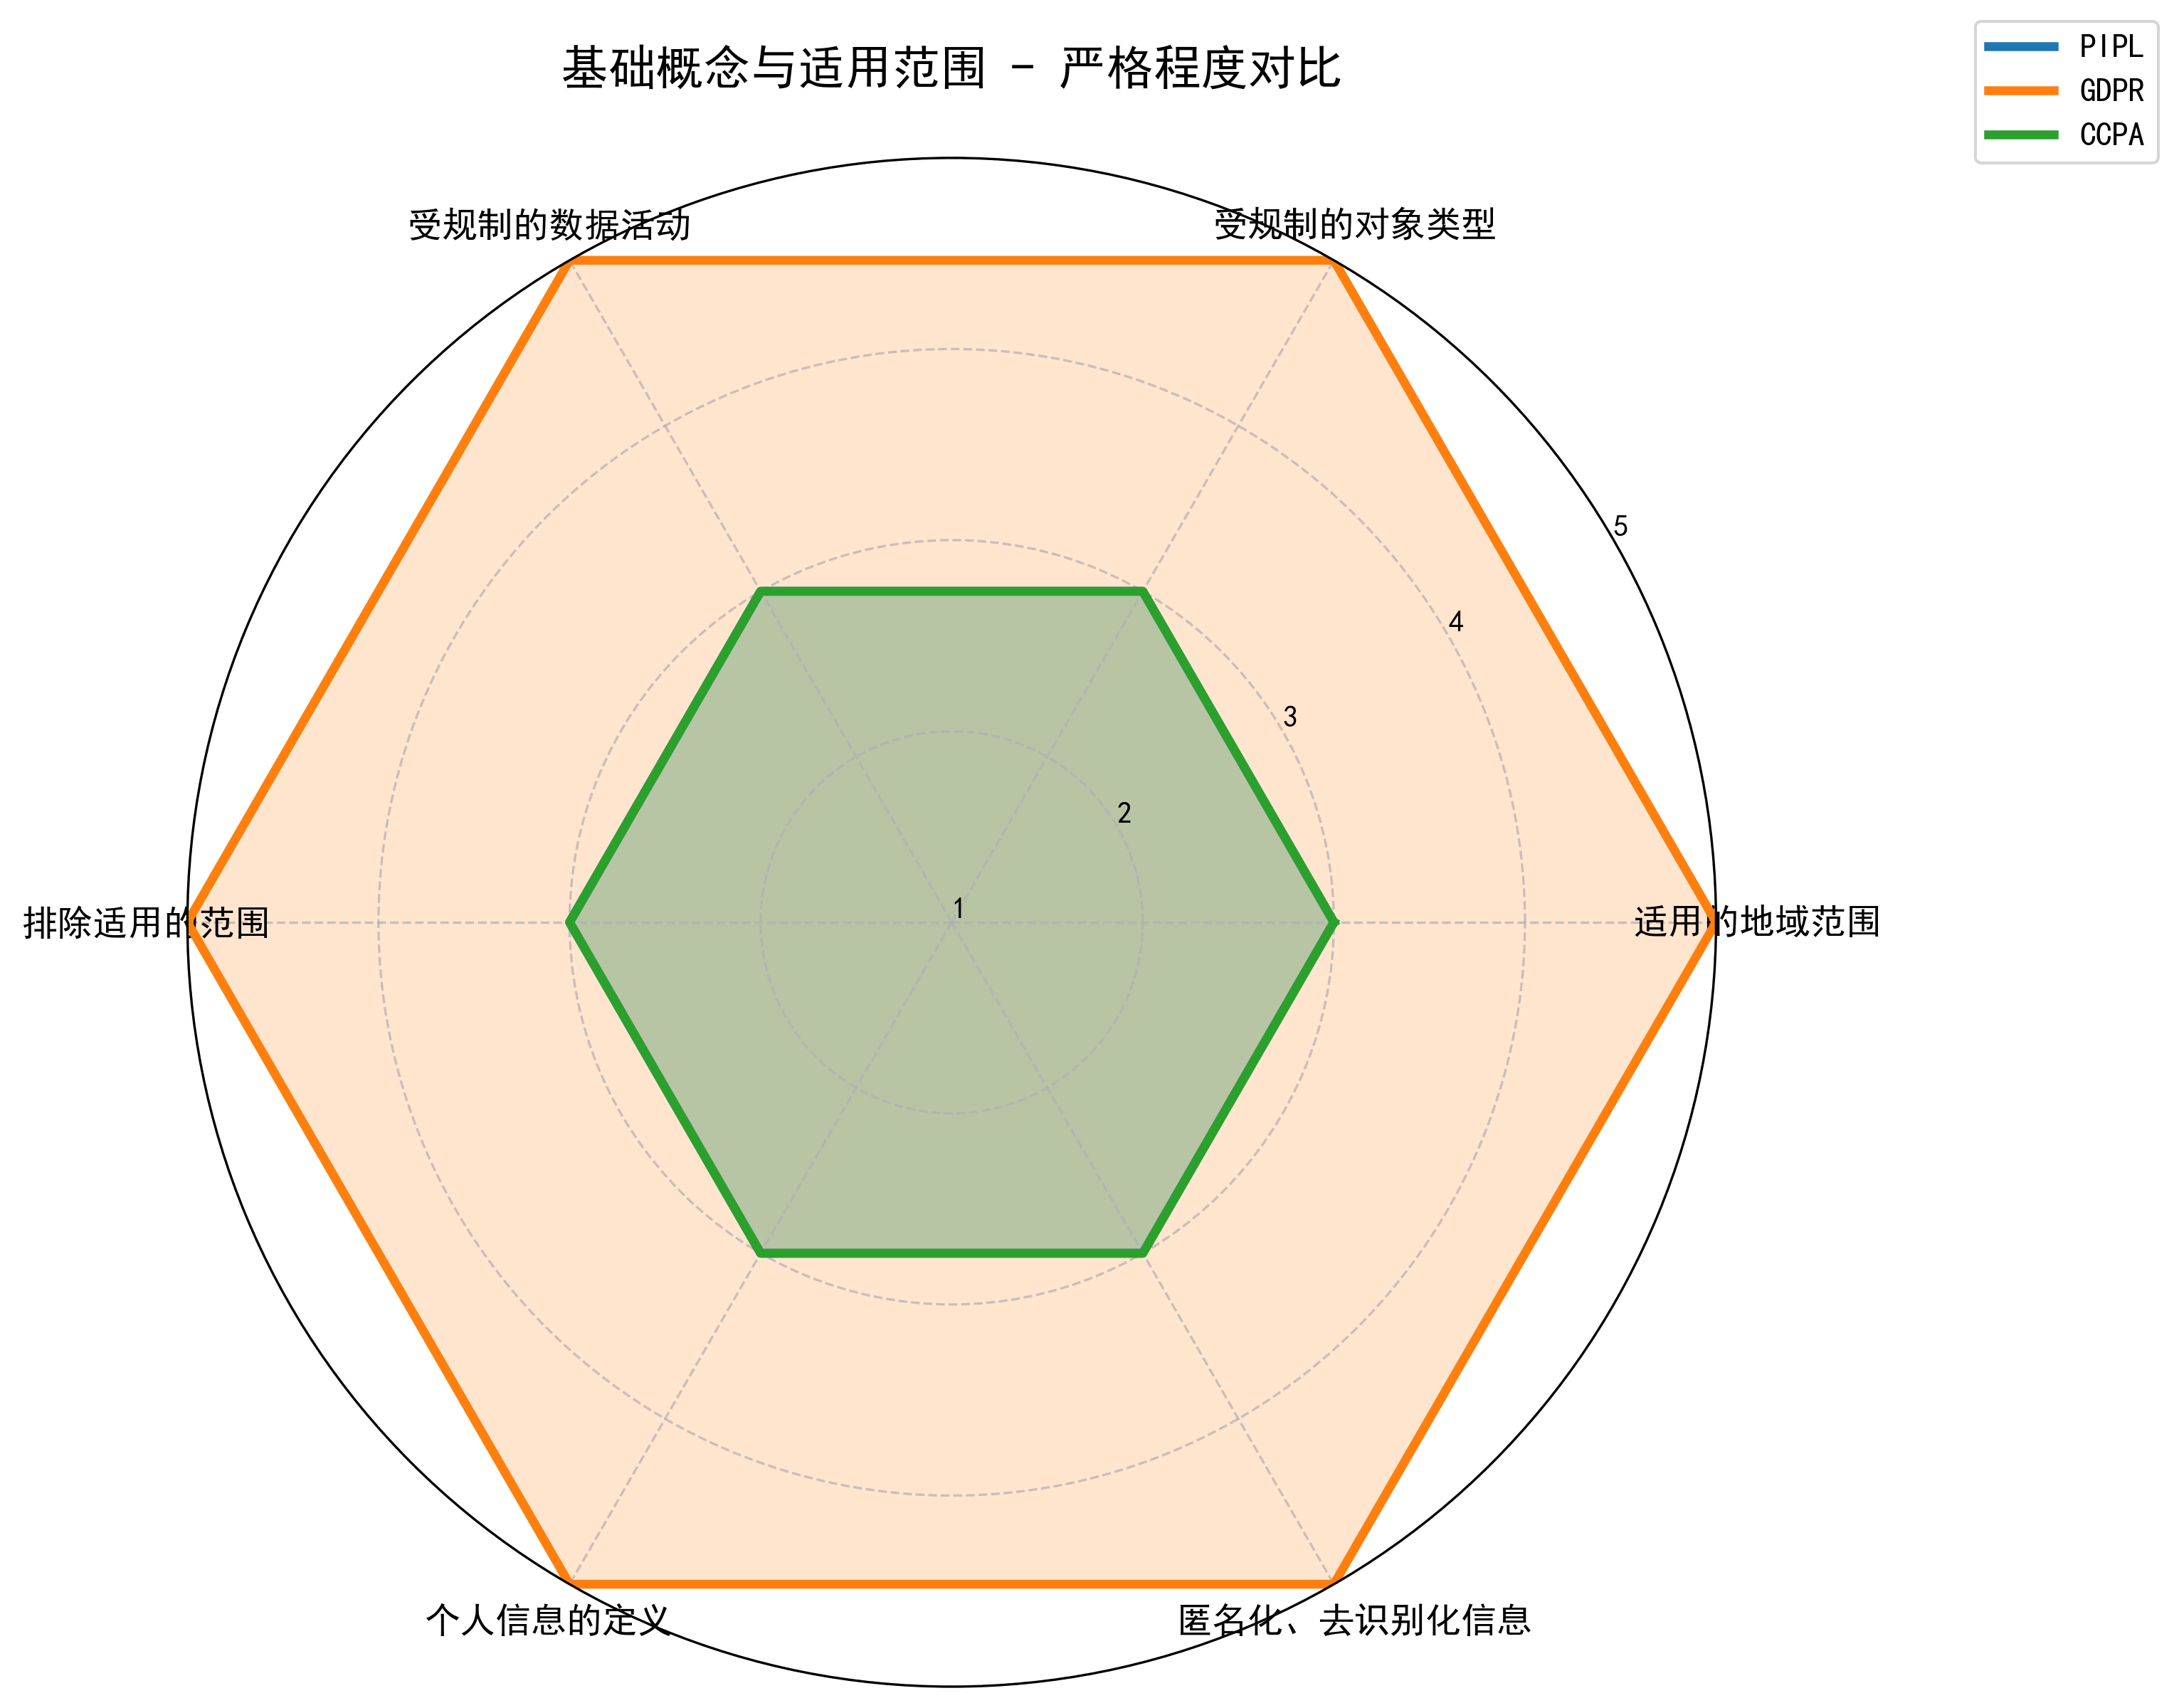
\includegraphics[width=0.8\textwidth]{pics/radar_基础概念与适用范围_strictness.png}
	\end{figure}
\end{frame}

\subsection{处理的核心原则与合法性}
\begin{frame}
	\frametitle{处理的核心原则与合法性}
	\footnotesize
	\begin{tabularx}{\textwidth}{X|X|X|X}
		\toprule
		\textbf{比较点} & \textbf{PIPL} & \textbf{GDPR} & \textbf{CCPA} \\
		\midrule
		合法性基础 & 7种（同意、合同、法定义务、公共事件、公共利益、已公开信息、其他）；无"正当利益" & 6种（同意、合同、法定义务、切身利益、公共任务、合法利益） & "告知+选择退出"模式，普通收集无需事前合法性基础 \\
		同意规则 & 自愿、明确、可撤回；特定场景需单独同意 & 自由给予、明确、知情、不含糊；可撤回；合同履行不得以不必要同意为条件 & 普通收集无需事前同意；向未成年人销售、金融激励等需Opt-in \\
		敏感个人信息 & 生物识别、医疗健康、金融账户、行踪轨迹、不满14周岁信息等；需单独同意+特定目的 & 特殊类别数据（种族、政治观点、基因、生物特征、健康、性取向等）原则上禁止处理 & 敏感个人信息（社保号、精准定位、种族等）；消费者可限制使用 \\
		\bottomrule
	\end{tabularx}
\end{frame}

\begin{frame}
	\frametitle{处理的核心原则与合法性}
	\footnotesize
	\begin{tabularx}{\textwidth}{X|X|X|X}
		\toprule
		\textbf{比较点} & \textbf{PIPL} & \textbf{GDPR} & \textbf{CCPA} \\
		\midrule
		未成年人信息 & 不满14周岁为敏感信息，需父母同意 & 16岁以下（成员国可降至13岁）需父母同意 & 16岁以下出售/共享需Opt-in；13岁以下需父母授权 \\
		死者信息 & 近亲属可为自身利益行使权利 & 序言明确不适用，成员国自定 & 未设专门规则 \\
		保存期限 & 实现目的的最短时间 & 存储限期原则，不超过目的所需 & 收集前告知保留时长或标准；不得超合理必要 \\
		\bottomrule
	\end{tabularx}
\end{frame}

\begin{frame}
	\frametitle{处理的核心原则与合法性 - 星级对比}
	\centering
	\textbf{作用范围星级对比}
	\begin{figure}
		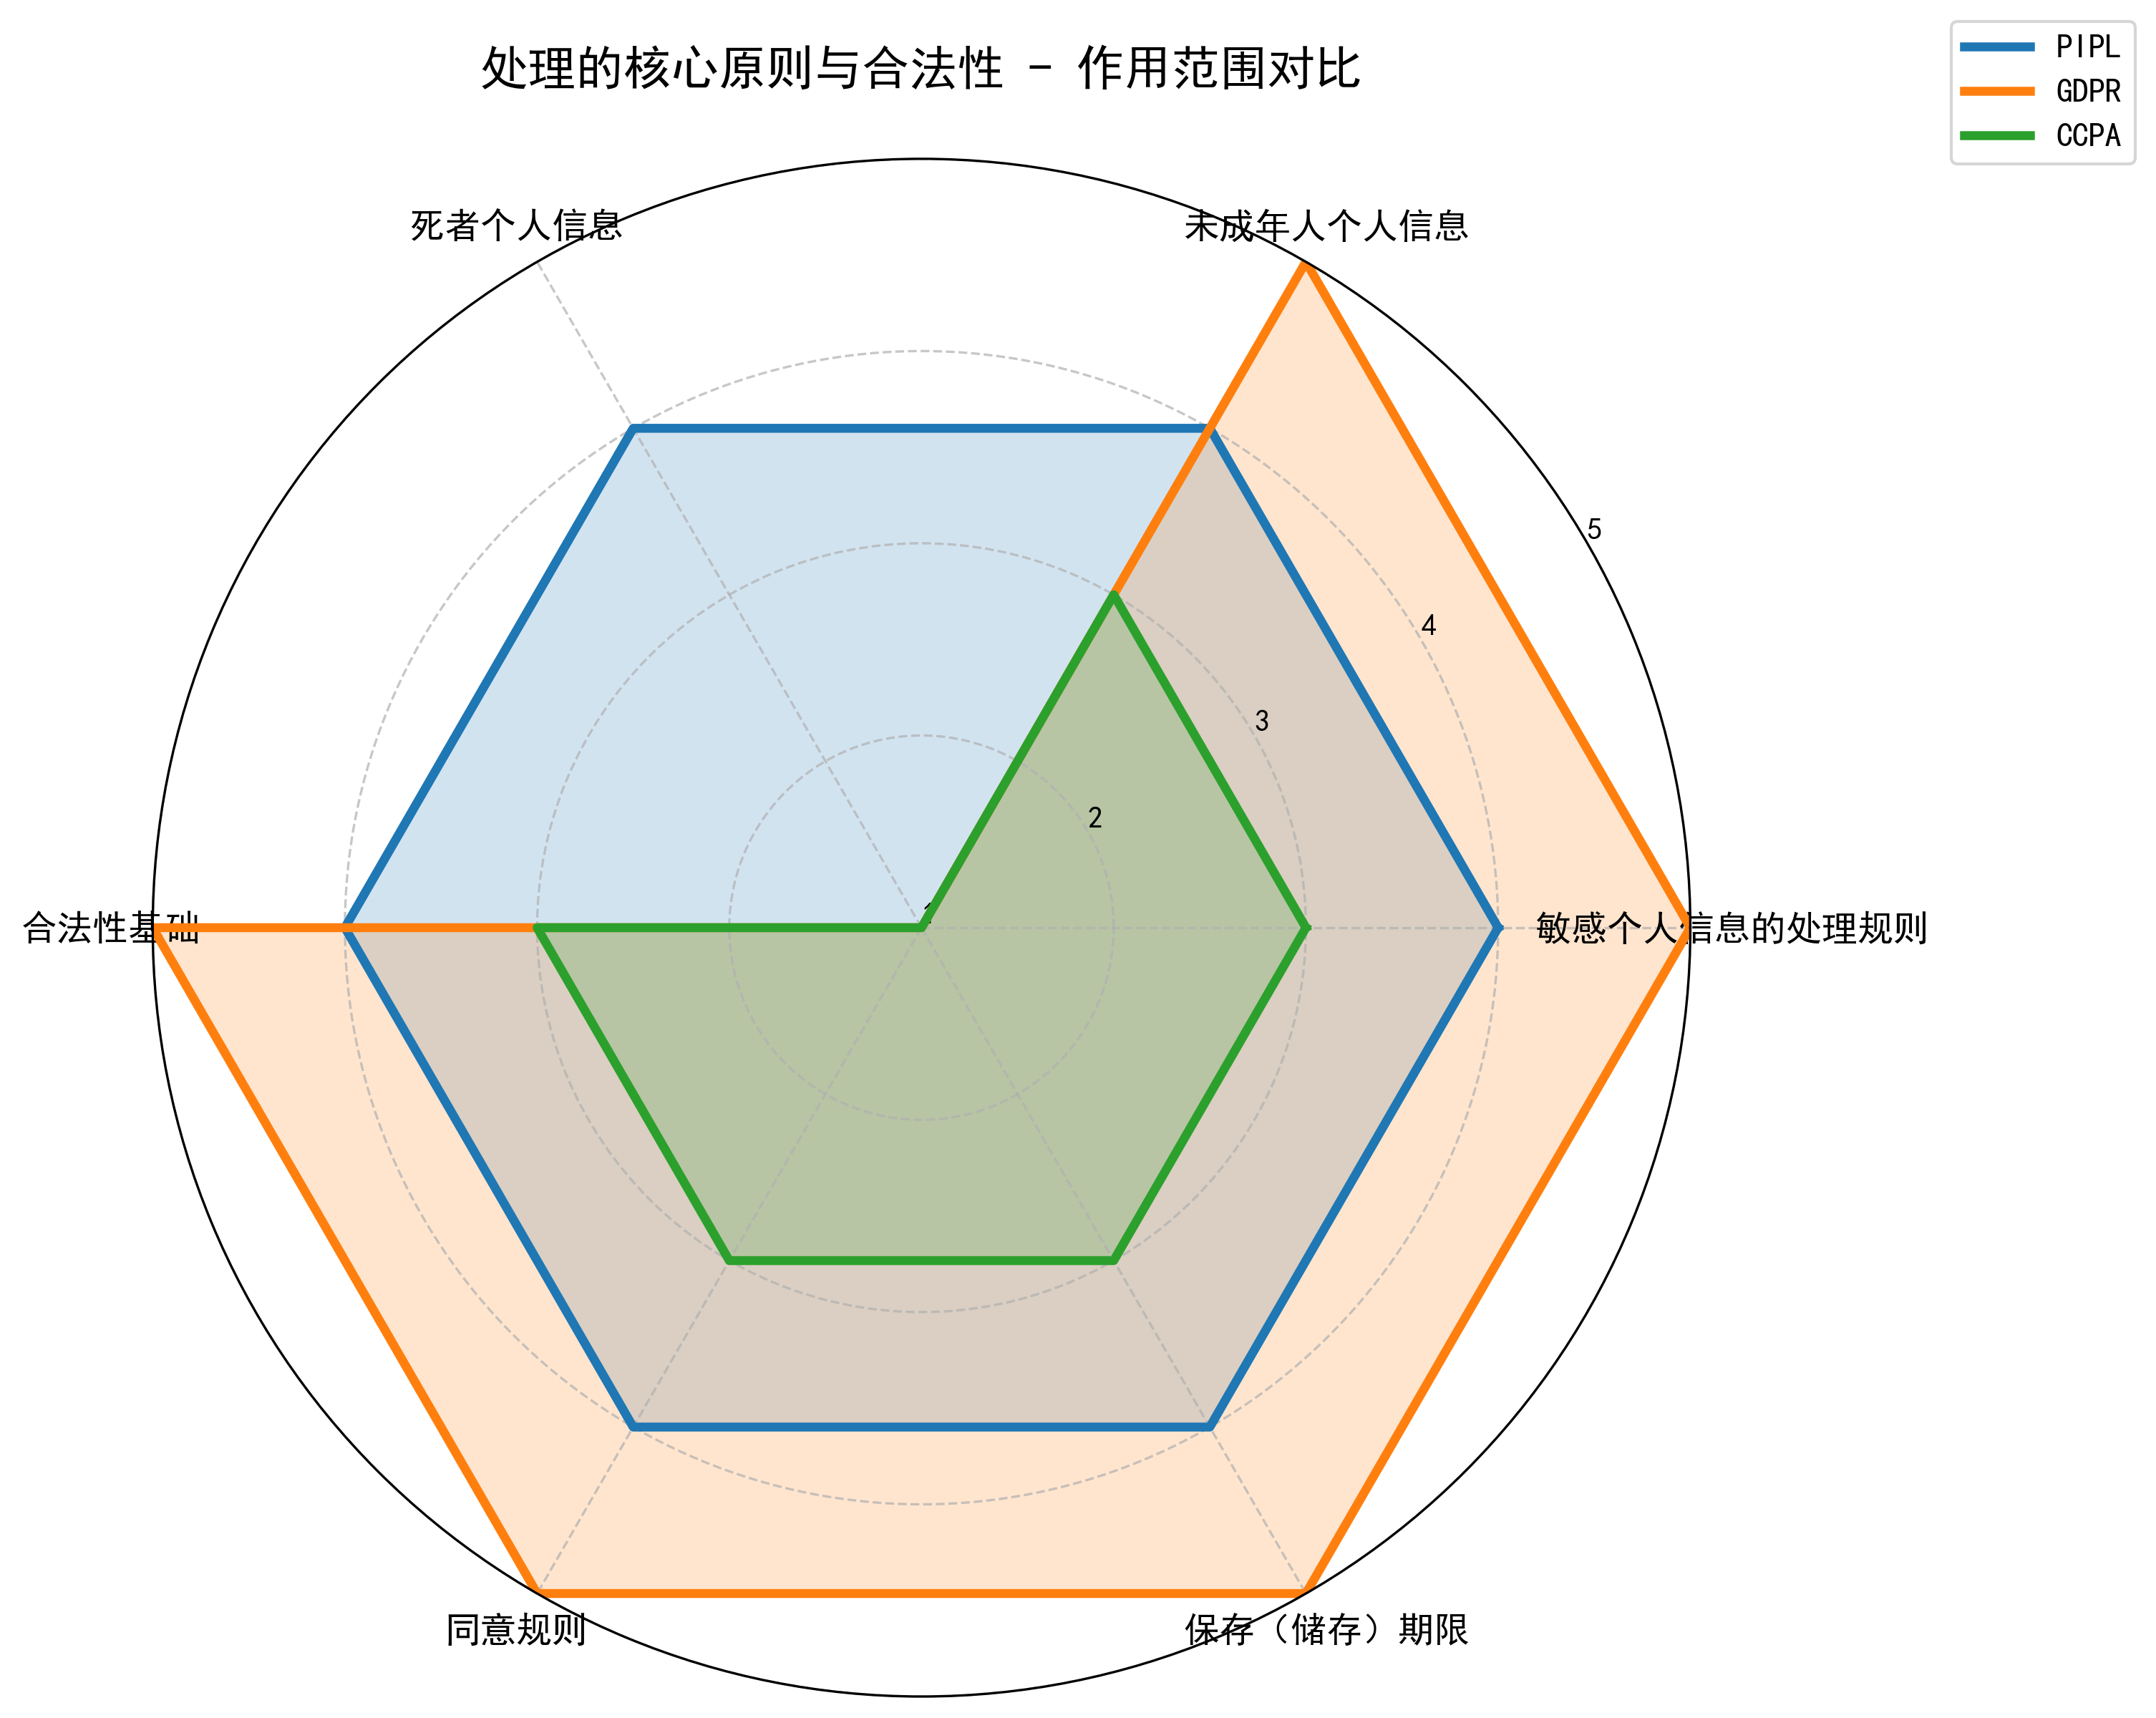
\includegraphics[width=0.8\textwidth]{pics/radar_处理的核心原则与合法性_scope.png}
	\end{figure}
\end{frame}

\begin{frame}
	\frametitle{处理的核心原则与合法性 - 星级对比}
	\centering
	\textbf{严格程度星级对比}
	\begin{figure}
		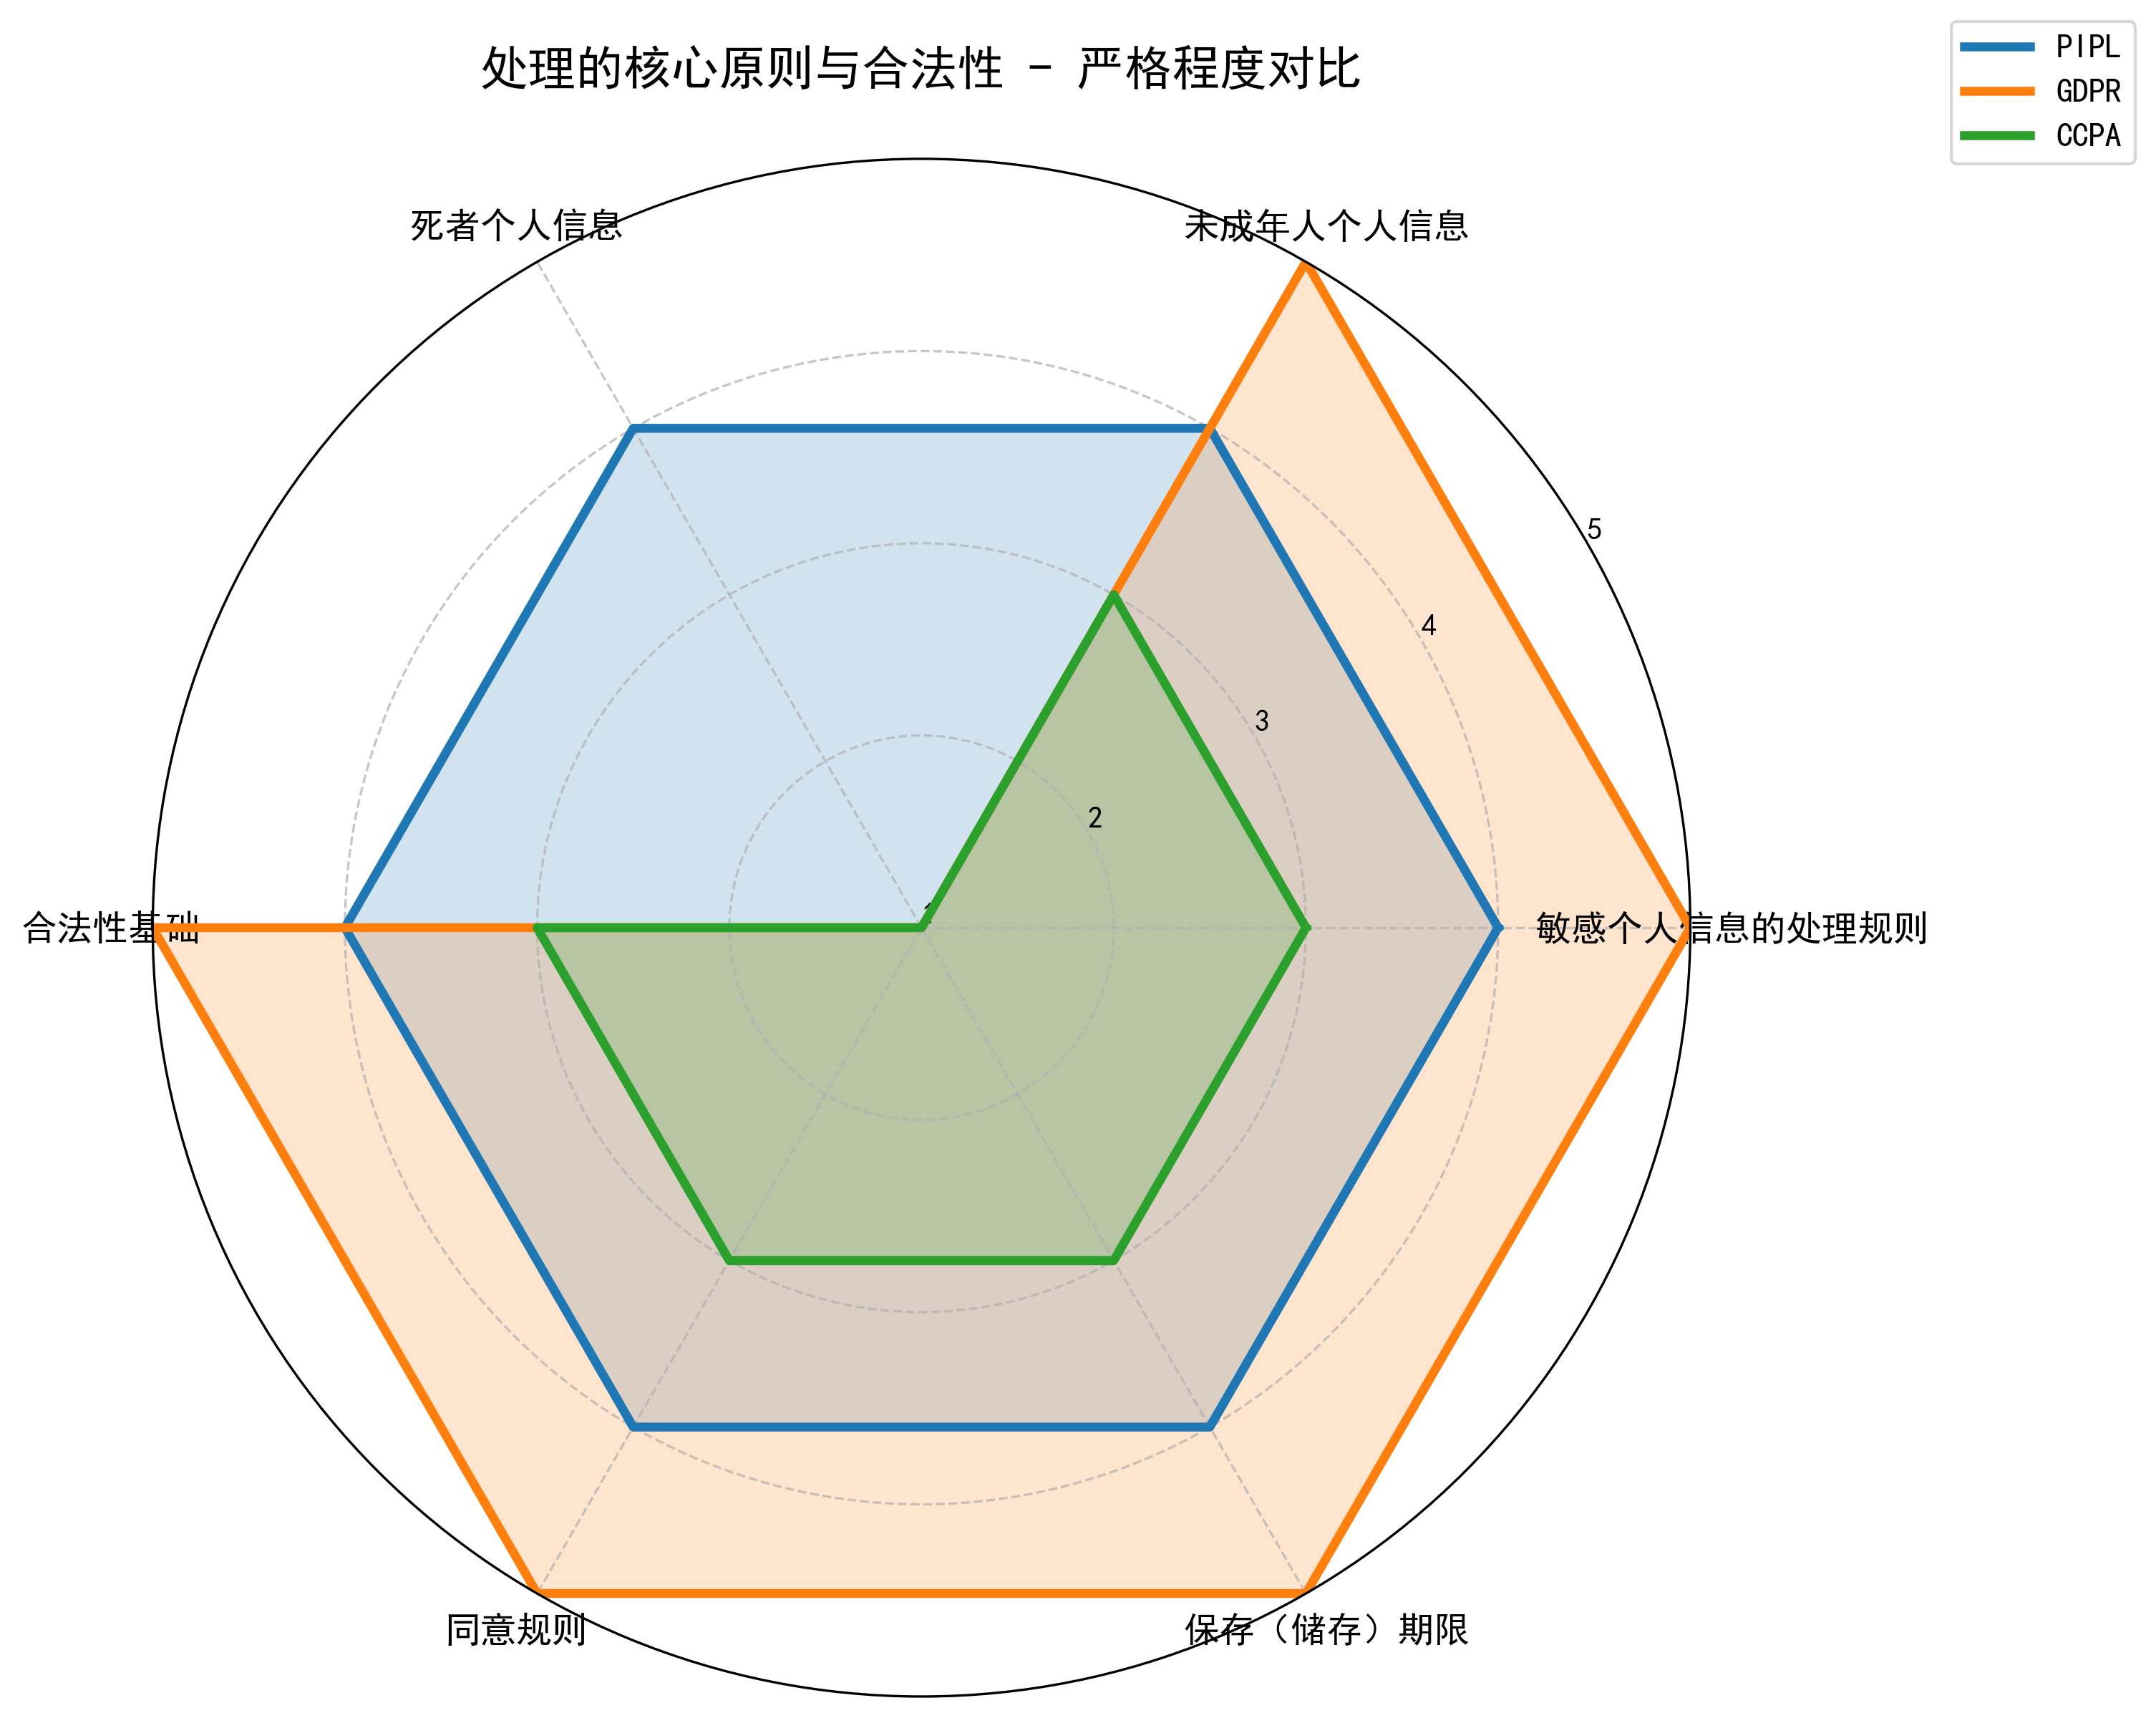
\includegraphics[width=0.8\textwidth]{pics/radar_处理的核心原则与合法性_strictness.png}
	\end{figure}
\end{frame}

\subsection{数据主体的权利}
\begin{frame}
	\frametitle{数据主体的权利}
	\footnotesize
	\begin{tabularx}{\textwidth}{X|X|X|X}
		\toprule
		\textbf{权利类型} & \textbf{PIPL} & \textbf{GDPR} & \textbf{CCPA} \\
		\midrule
		知情权 & 处理目的、方式、种类等以显著方式告知 & 以简洁透明方式告知处理目的、法律依据等 & 收集时告知信息类别和用途 \\
		访问/复制权 & 有权查阅、复制 & 有权访问个人信息及处理信息 & 有权要求披露收集的具体信息 \\
		更正权 & 有权请求更正 & 有权要求及时更正 & 2026年生效条款赋予更正权 \\
		删除权 & 5种情形（目的实现、停止服务、期限届满、撤回同意、违法处理） & 适用范围最广（数据不再必要、撤回同意、反对、非法处理等） & 有权要求删除，但例外较多（完成交易、安全、言论自由、科研等） \\
		可携权 & 需符合国家网信部门规定（未完全落地） & 以结构化、通用、机器可读格式获取，并可无障碍传输 & 有权获取便携格式，2026年新规明确"便于传输" \\
		\bottomrule
	\end{tabularx}
\end{frame}

\begin{frame}
	\frametitle{数据主体的权利}
	\footnotesize
	\begin{tabularx}{\textwidth}{X|X|X|X}
		\toprule
		\textbf{权利类型} & \textbf{PIPL} & \textbf{GDPR} & \textbf{CCPA} \\
		\midrule
		限制处理权 & 无 & 有（质疑准确性期间、非法处理但反对删除等） & 无 \\
		自动化决策相关 & 反杀熟；对重大影响决定可拒绝 & 不受制于仅自动化决策；例外需人工干预 & 2026年新规：有权选择退出自动化决策技术（ADMT） \\
		已公开信息处理 & 可合理范围处理，个人明确拒绝除外 & 无专门条款，需合法性基础 & 无专门规则 \\
		逝者信息权利 & 近亲属可为自身利益行使权利 & 不适用 & 无 \\
		\bottomrule
	\end{tabularx}
\end{frame}

\begin{frame}
	\frametitle{数据主体的权利 - 星级对比}
	\centering
	\textbf{作用范围星级对比}
	\begin{figure}
		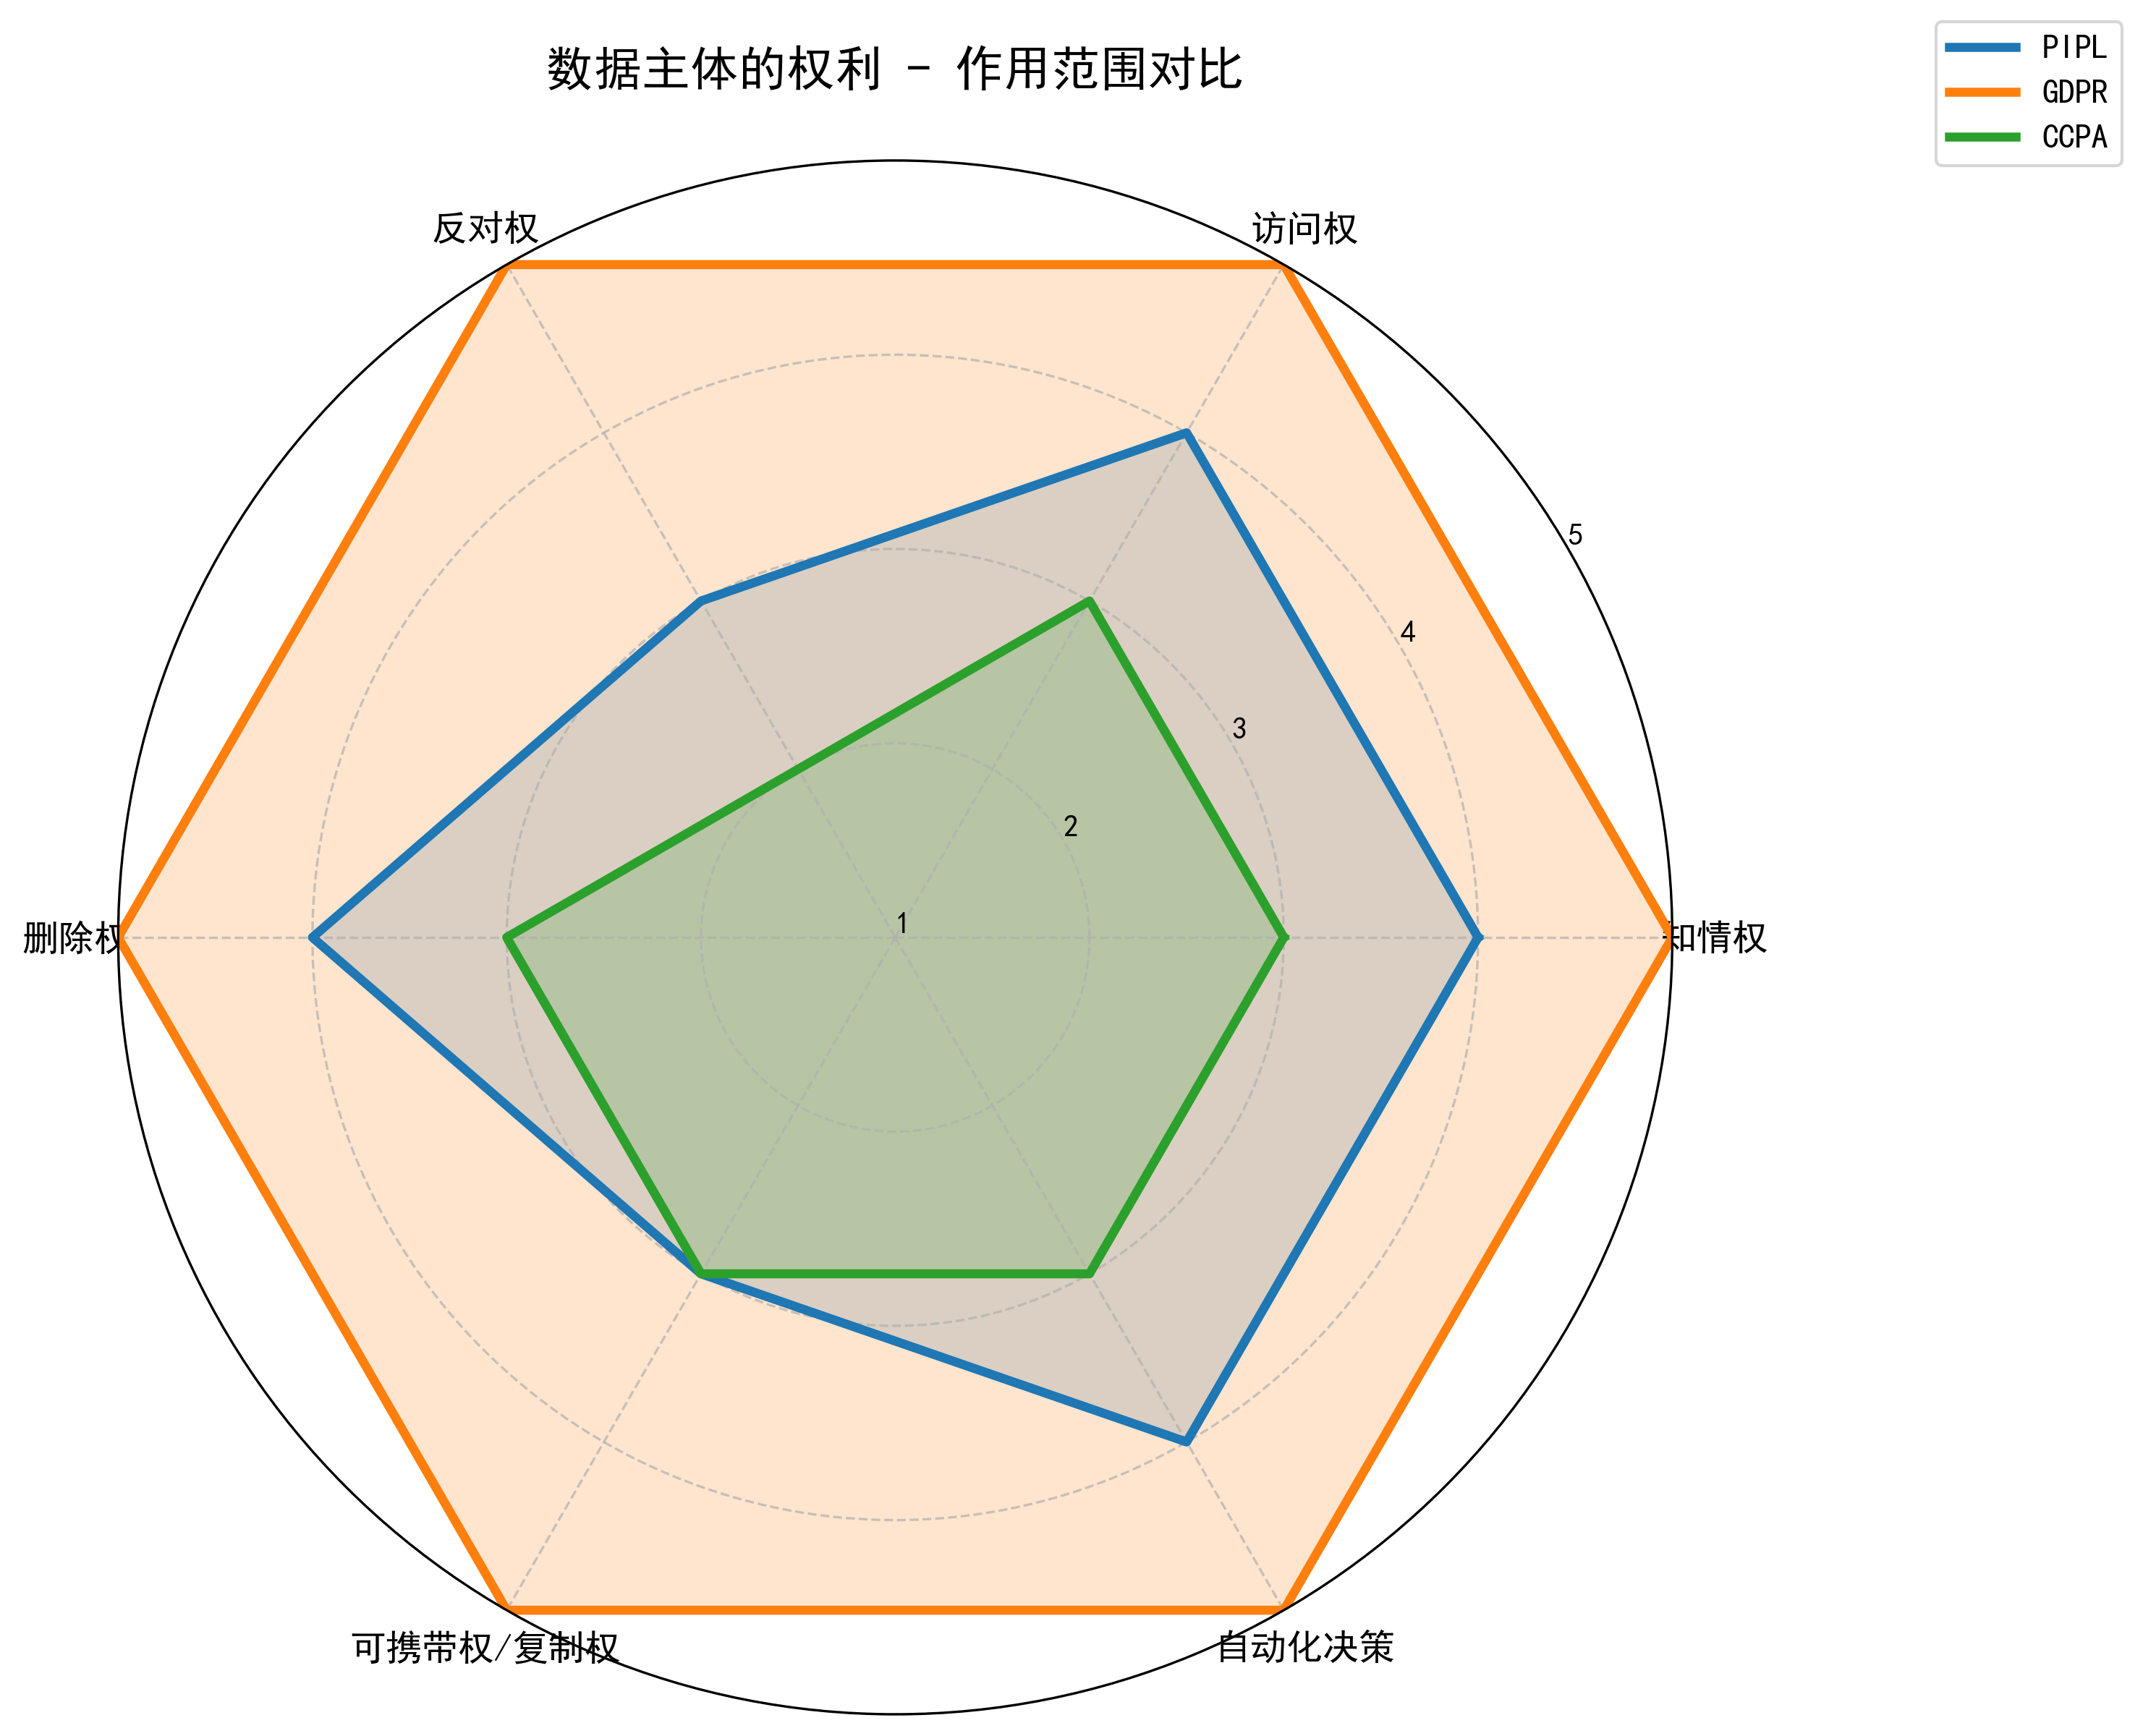
\includegraphics[width=0.8\textwidth]{pics/radar_数据主体的权利_scope.png}
	\end{figure}
	
\end{frame}

\begin{frame}
	\frametitle{数据主体的权利 - 星级对比}
	\centering
	
	\textbf{严格程度星级对比}
	\begin{figure}
		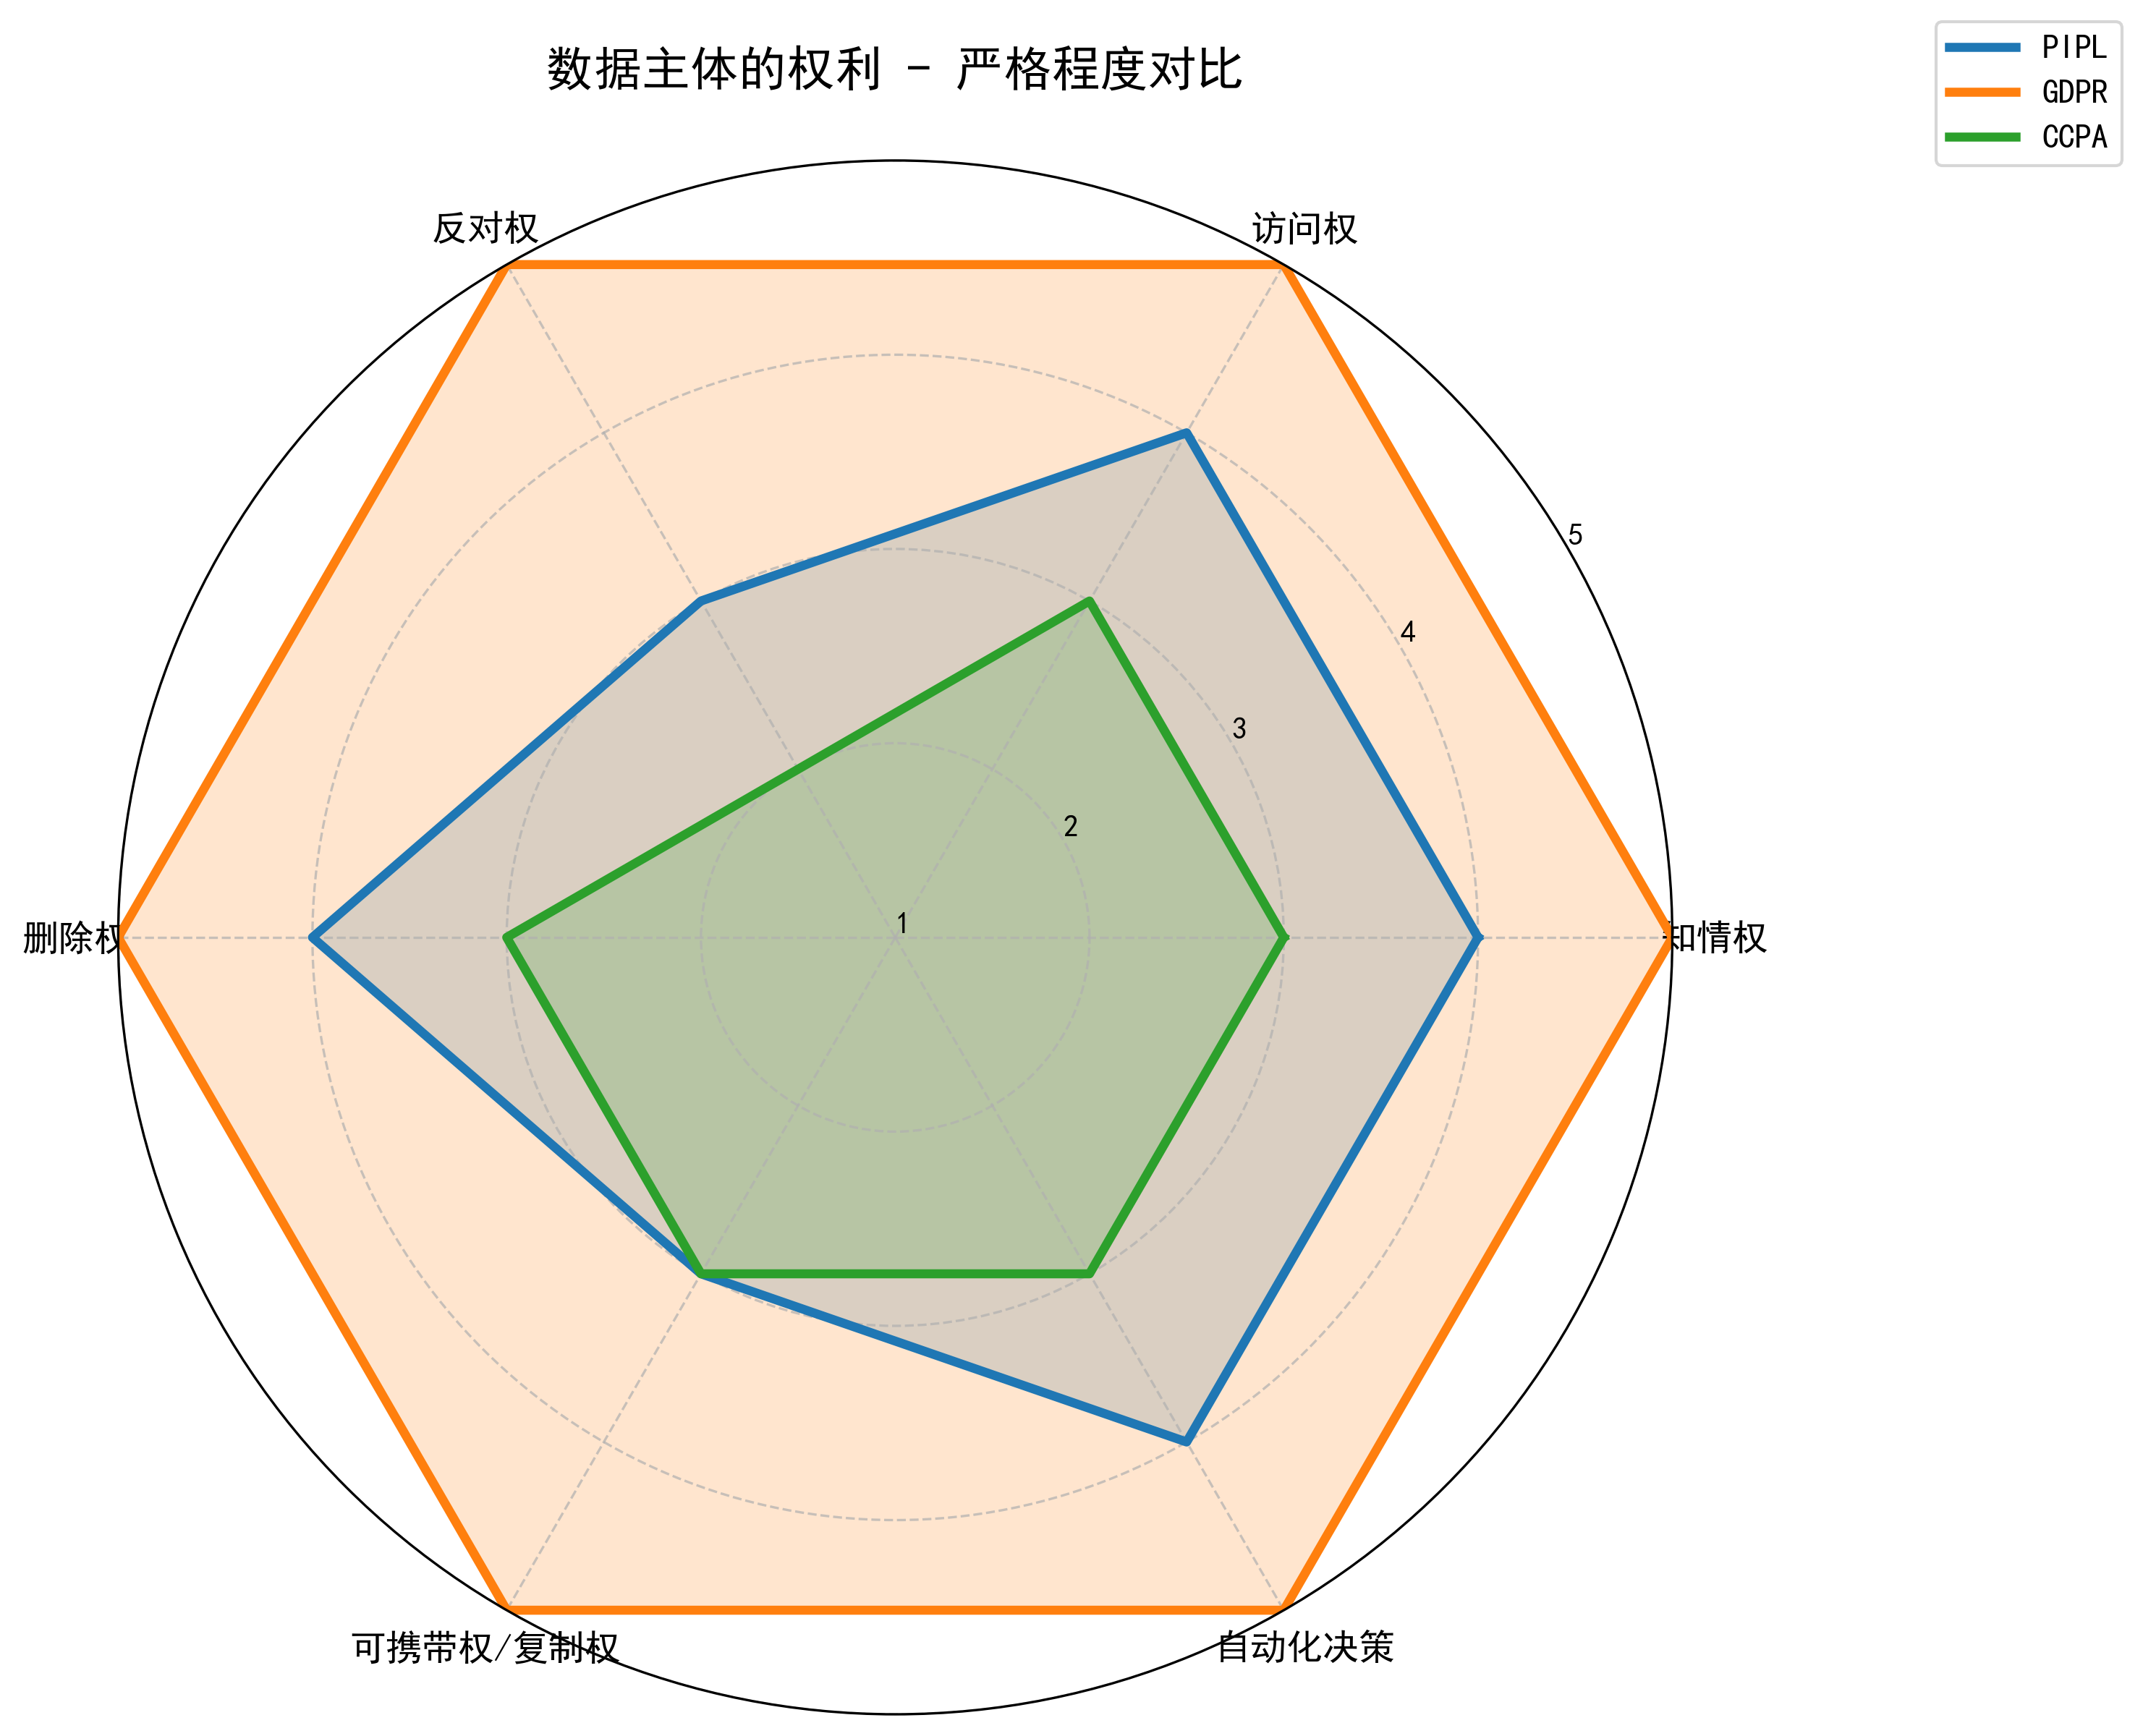
\includegraphics[width=0.8\textwidth]{pics/radar_数据主体的权利_strictness.png}
	\end{figure}
\end{frame}

\subsection{处理者的义务与合规}
\begin{frame}
	\frametitle{处理者的义务与合规}
	\footnotesize
	\begin{tabularx}{\textwidth}{X|X|X|X}
		\toprule
		\textbf{义务类型} & \textbf{PIPL} & \textbf{GDPR} & \textbf{CCPA} \\
		\midrule
		安全保障措施 & 加密、去标识化、权限管理、应急预案等 & 假名化、加密、保密性、恢复能力、定期测试等 & 合理安全程序；2026年新规对"重大风险"企业强制网络安全审计 \\
		数据安全事件通知 & 立即补救并通知；未规定具体小时 & 72小时内通知监管机构；高风险泄露需通知个人 & 加州民法典：最迟15天内通知受影响个人 \\
		个人信息保护影响评估 & 处理敏感信息、出境等需评估，报告保存3年 & 高风险处理需DPIA；风险无法缓解需事前咨询监管机构 & 处理敏感信息、使用ADMT、出售/共享信息需隐私风险评估 \\
		DPO/负责人指定 & 达到规定数量需指定负责人，报送监管部门；境外处理者需境内代表 & 公共机构、大规模监控、大规模敏感数据处理必须指定DPO，独立性保护 & 无强制DPO要求，仅需联系方式 \\
		\bottomrule
	\end{tabularx}
\end{frame}

\begin{frame}
	\frametitle{处理者的义务与合规}
	\footnotesize
	\begin{tabularx}{\textwidth}{X|X|X|X}
		\toprule
		\textbf{义务类型} & \textbf{PIPL} & \textbf{GDPR} & \textbf{CCPA} \\
		\midrule
		守门人条款 & 重要互联网平台需设独立监督机构、公平规则、停止严重违法服务、发布社会责任报告 & 无直接对应条款（由DMA单独规定） & 无直接对应条款，但通过门槛管辖大型企业 \\
		自动化决策规制义务 & 保证公平、禁止杀熟；提供不针对个人特征的选项 & 保障人工干预、表达观点、提出异议 & 披露逻辑；提供选择退出权；进行风险评估 \\
		公共场所图像采集 & 安装设备须为公共安全必需，显著提示，信息只能用于公共安全目的 & 无专门条款，通过生物识别规则间接约束 & 无专门条款，但生物识别信息作为敏感信息处理 \\
		\bottomrule
	\end{tabularx}
\end{frame}

\begin{frame}
	\frametitle{处理者的义务与合规 - 星级对比}
	\centering
	\textbf{作用范围星级对比}
	\begin{figure}
		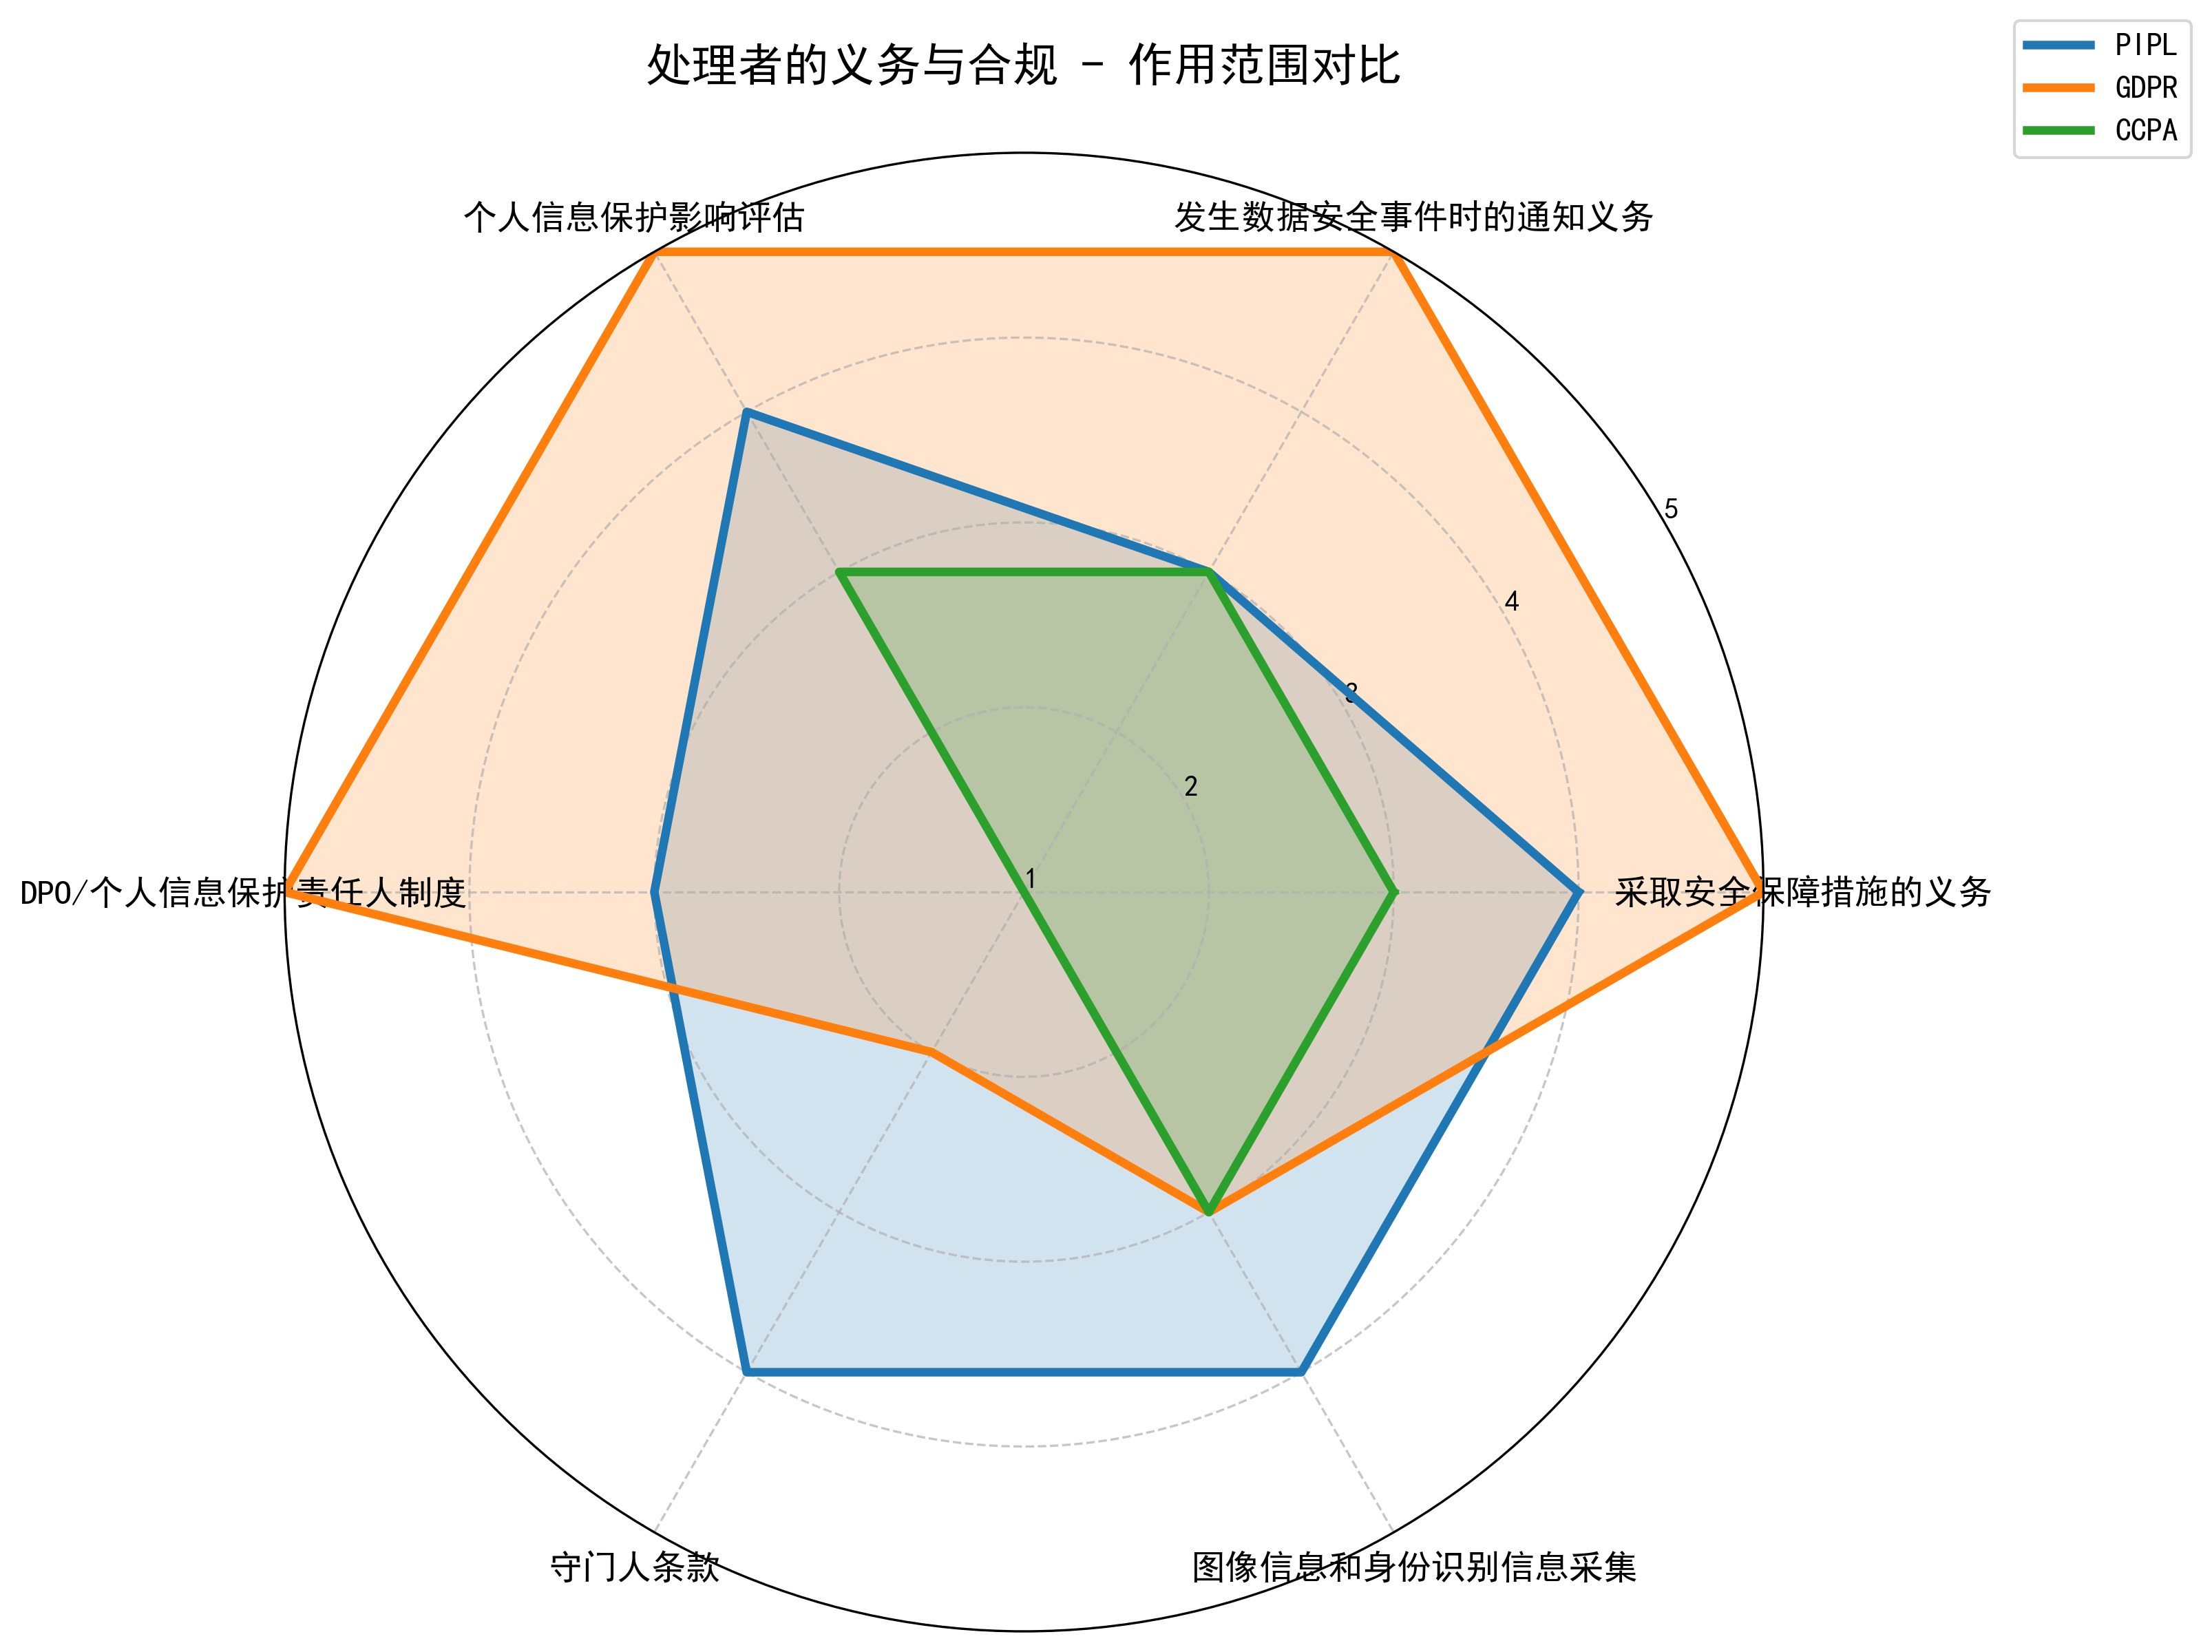
\includegraphics[width=0.8\textwidth]{pics/radar_处理者的义务与合规_scope.png}
	\end{figure}
\end{frame}

\begin{frame}
	\frametitle{处理者的义务与合规 - 星级对比}
	\centering
	
	\textbf{严格程度星级对比}
	\begin{figure}
		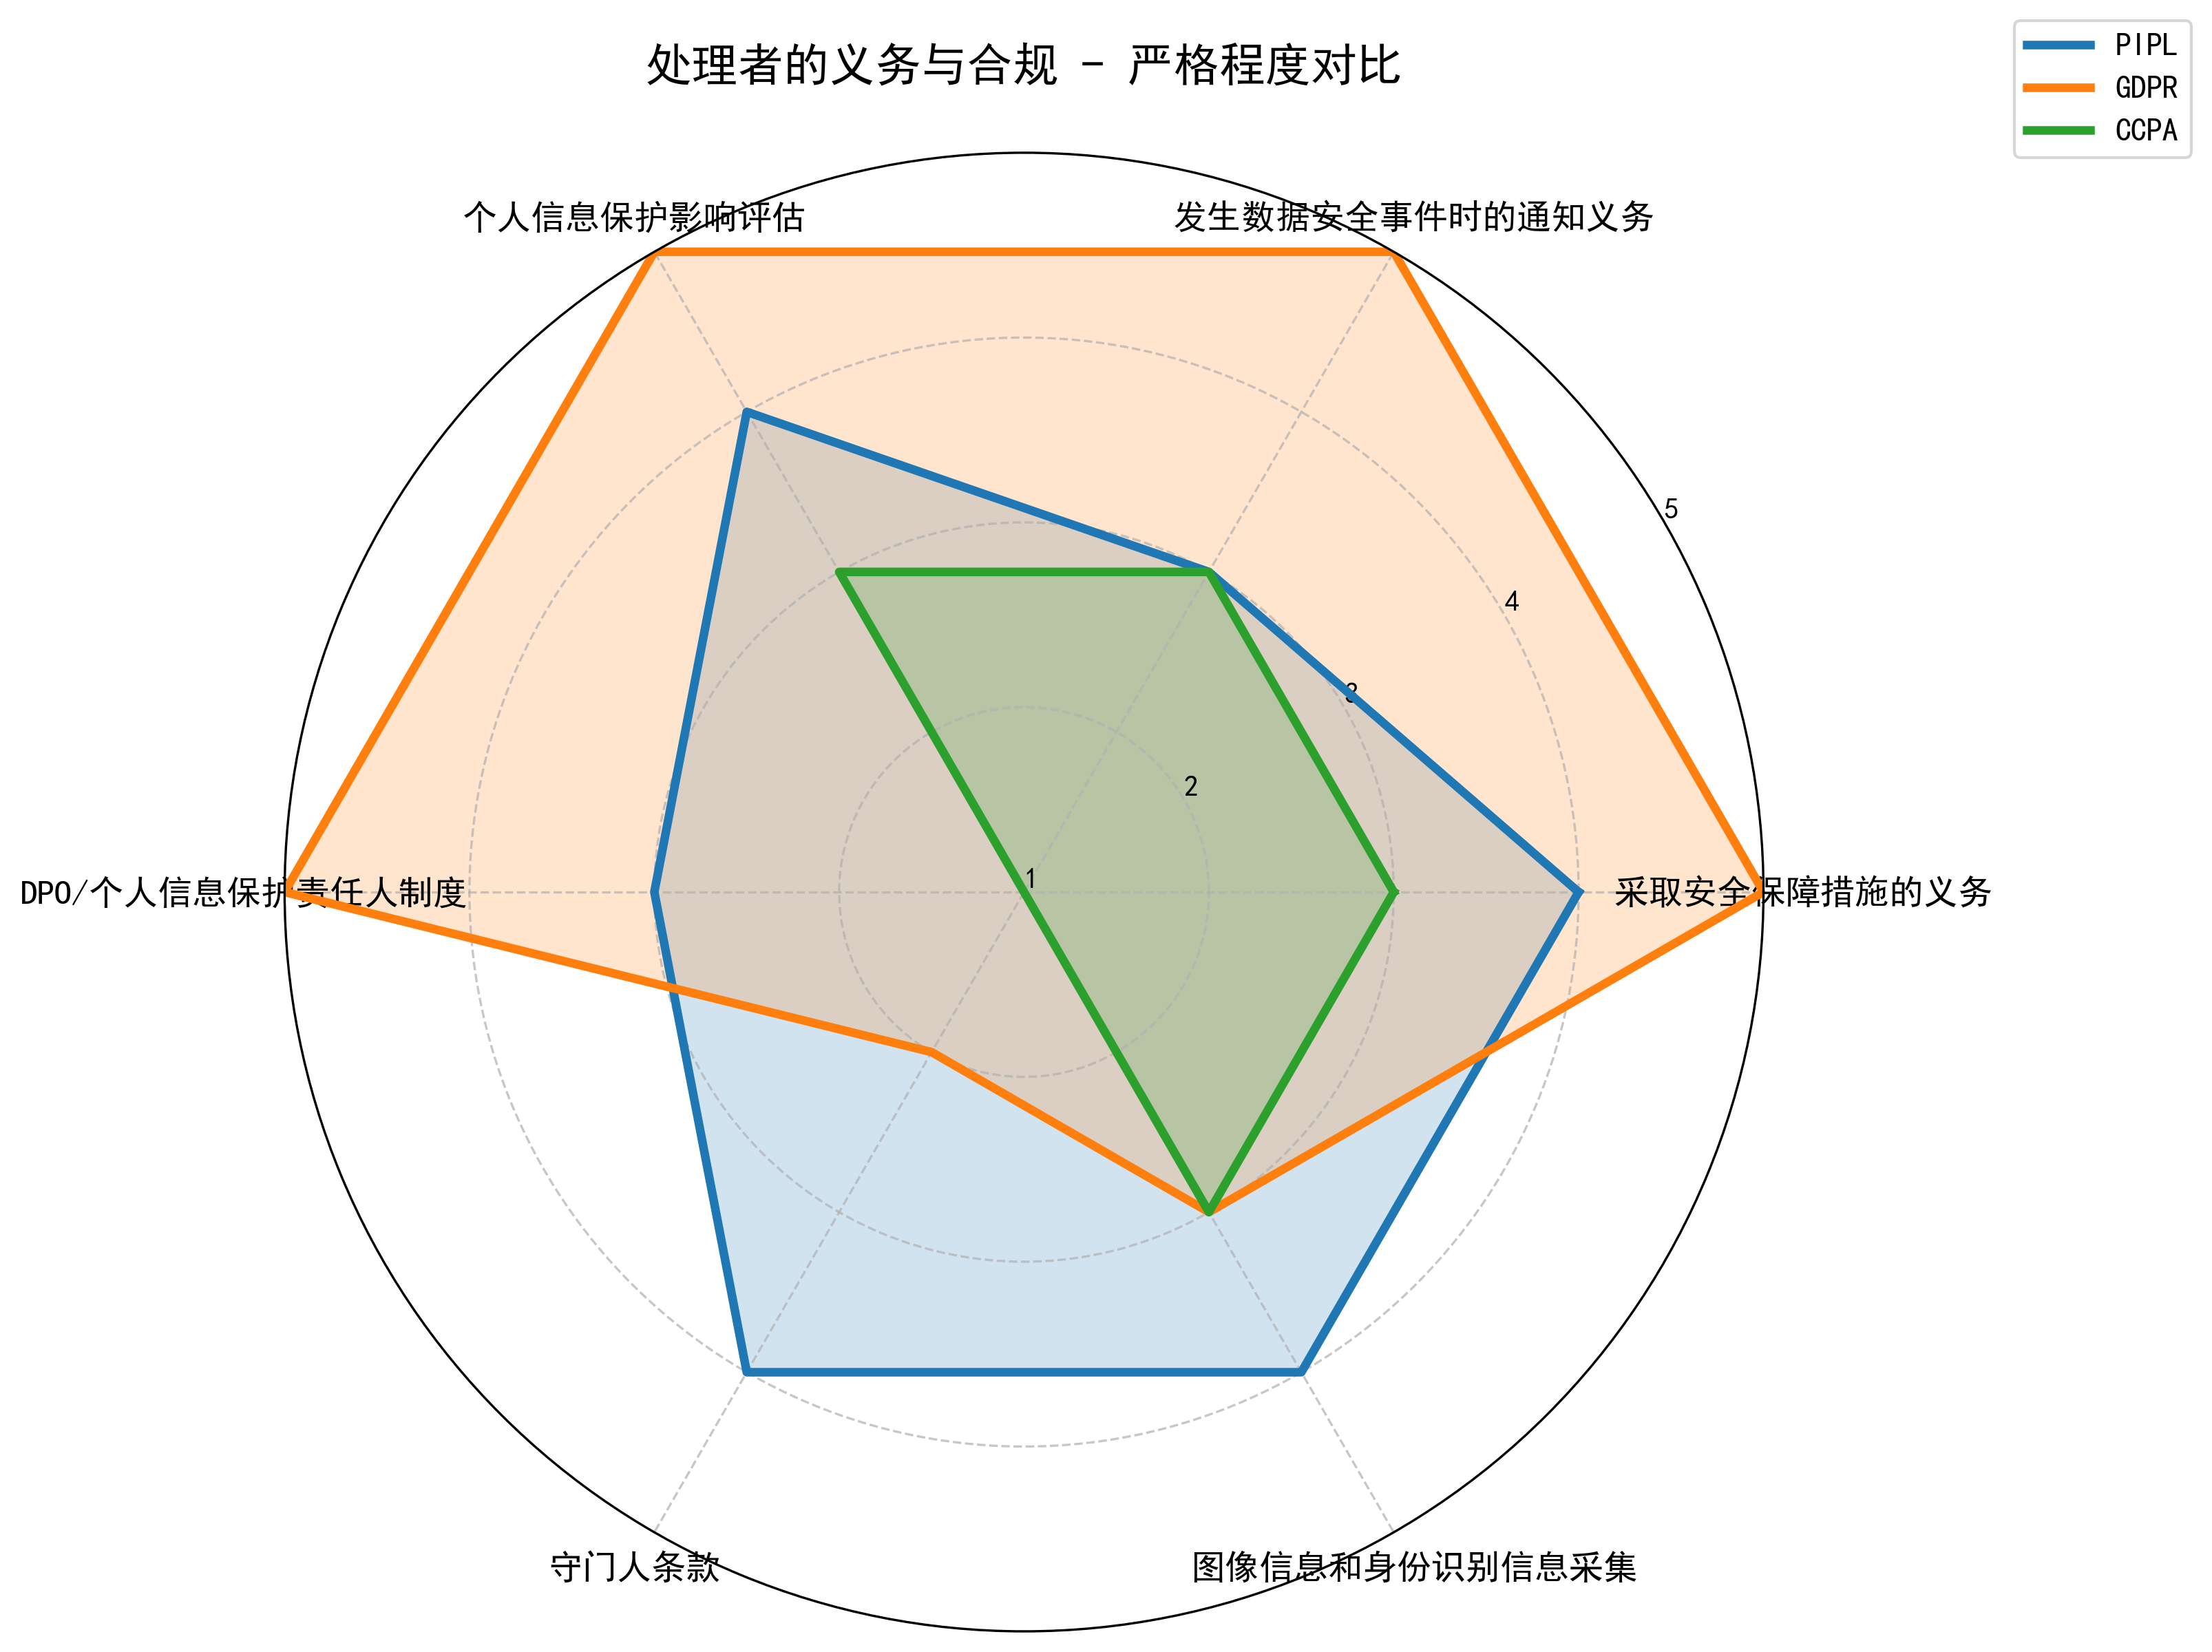
\includegraphics[width=0.8\textwidth]{pics/radar_处理者的义务与合规_strictness.png}
	\end{figure}
\end{frame}


\subsection{数据的跨境流动}
\begin{frame}
	\frametitle{数据的跨境流动}
	\footnotesize
	\begin{tabularx}{\textwidth}{X|X|X|X}
		\toprule
		\textbf{比较点} & \textbf{PIPL} & \textbf{GDPR} & \textbf{CCPA} \\
		\midrule
		是否设专章 & 是（第三章） & 是（第五章） & 否 \\
		充分性认定 & 无，但有类似机制（安全评估、认证、标准合同） & 有（欧盟委员会认定） & 无 \\
		传输机制 & 安全评估、认证、标准合同、其他条件 & 充分性认定、适当保障措施（SCC、BCR、行为准则、认证）、克减条款 & 对"向第三方披露"的合同要求 \\
		合同要求 & 与境外接收方订立标准合同 & SCC需欧盟批准；BCR需监管批准 & 书面合同，限制目的，要求同等保护 \\
		对境外接收方的态度 & 严格限制，关键设施和大量数据需境内存储 & 严格限制，必须确保保护水平不降低 & 无额外限制，适用相同合同义务 \\
		特殊机制 & 关键设施境内存储、对等原则、外国执法请求需批准 & 充分性认定；BCR；SCC；克减条款 & 若构成"出售"或"共享"，需提供选择退出权 \\
		\bottomrule
	\end{tabularx}
\end{frame}

\begin{frame}
	\frametitle{数据的跨境流动 - 星级对比}
	\centering
	\textbf{作用范围星级对比}
	\begin{figure}
		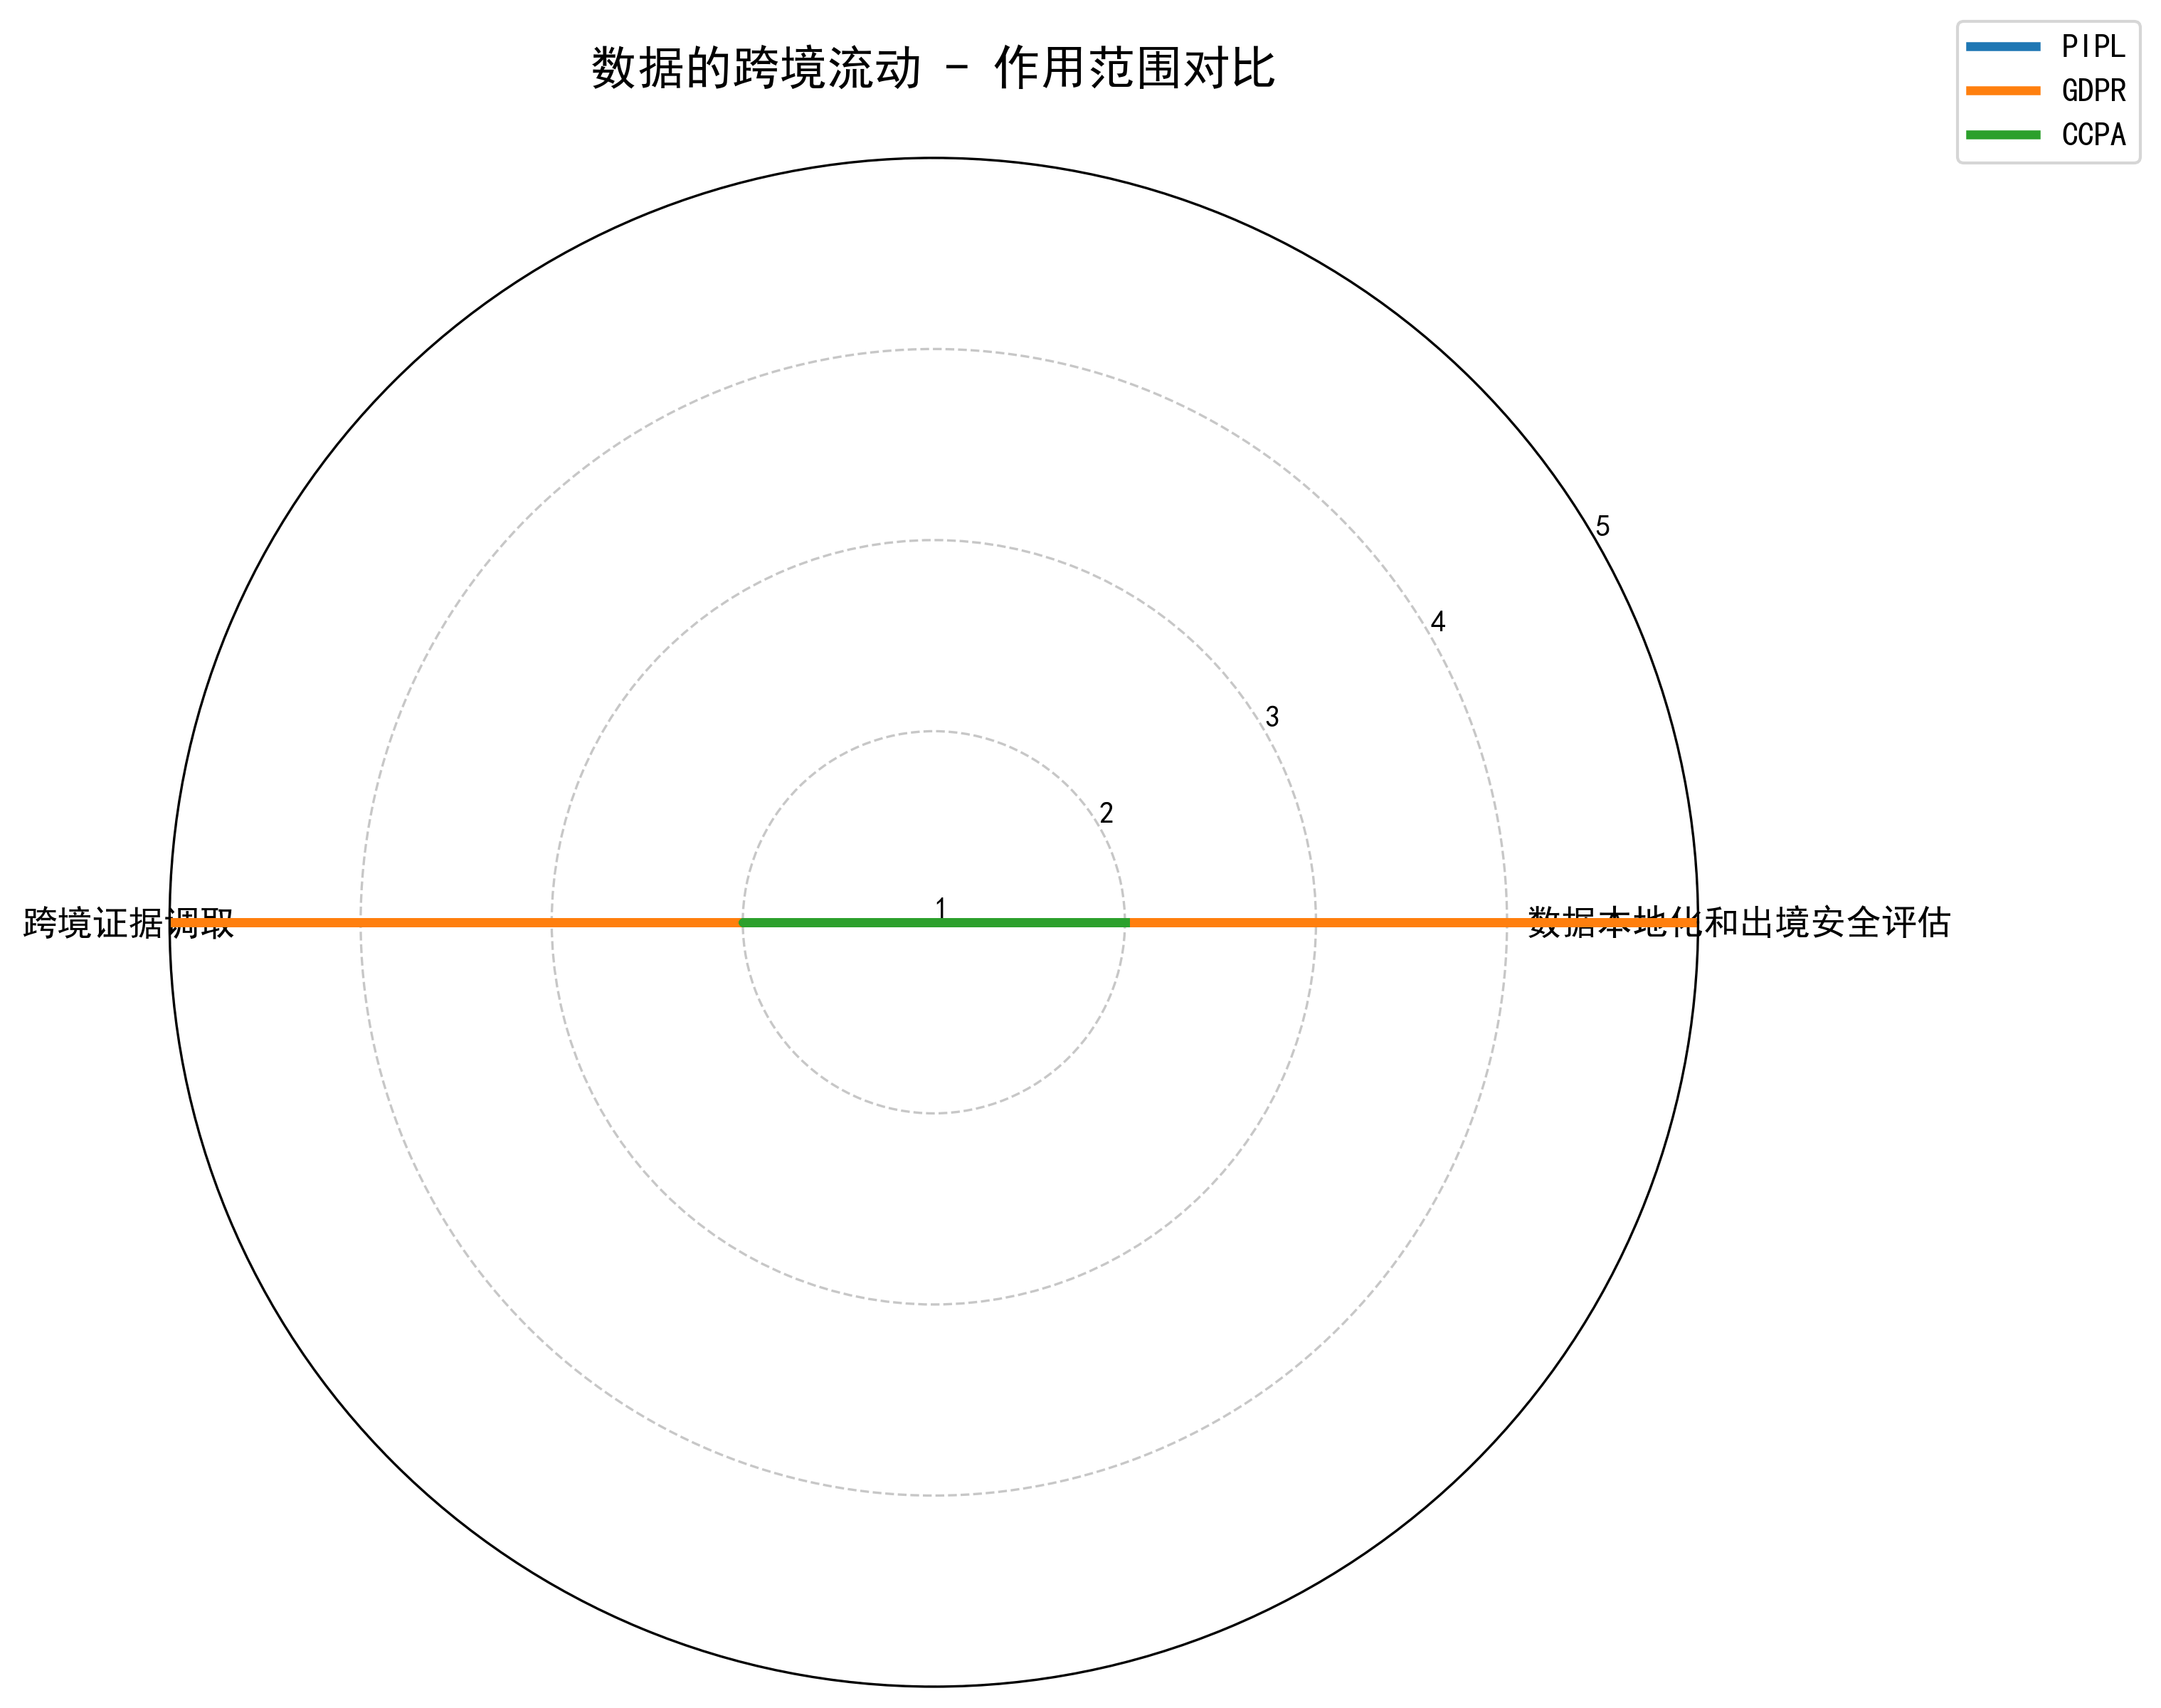
\includegraphics[width=0.8\textwidth]{pics/radar_数据的跨境流动_scope.png}
	\end{figure}

\end{frame}

\begin{frame}
	\frametitle{数据的跨境流动 - 星级对比}
	\centering
	
	\textbf{严格程度星级对比}
	\begin{figure}
		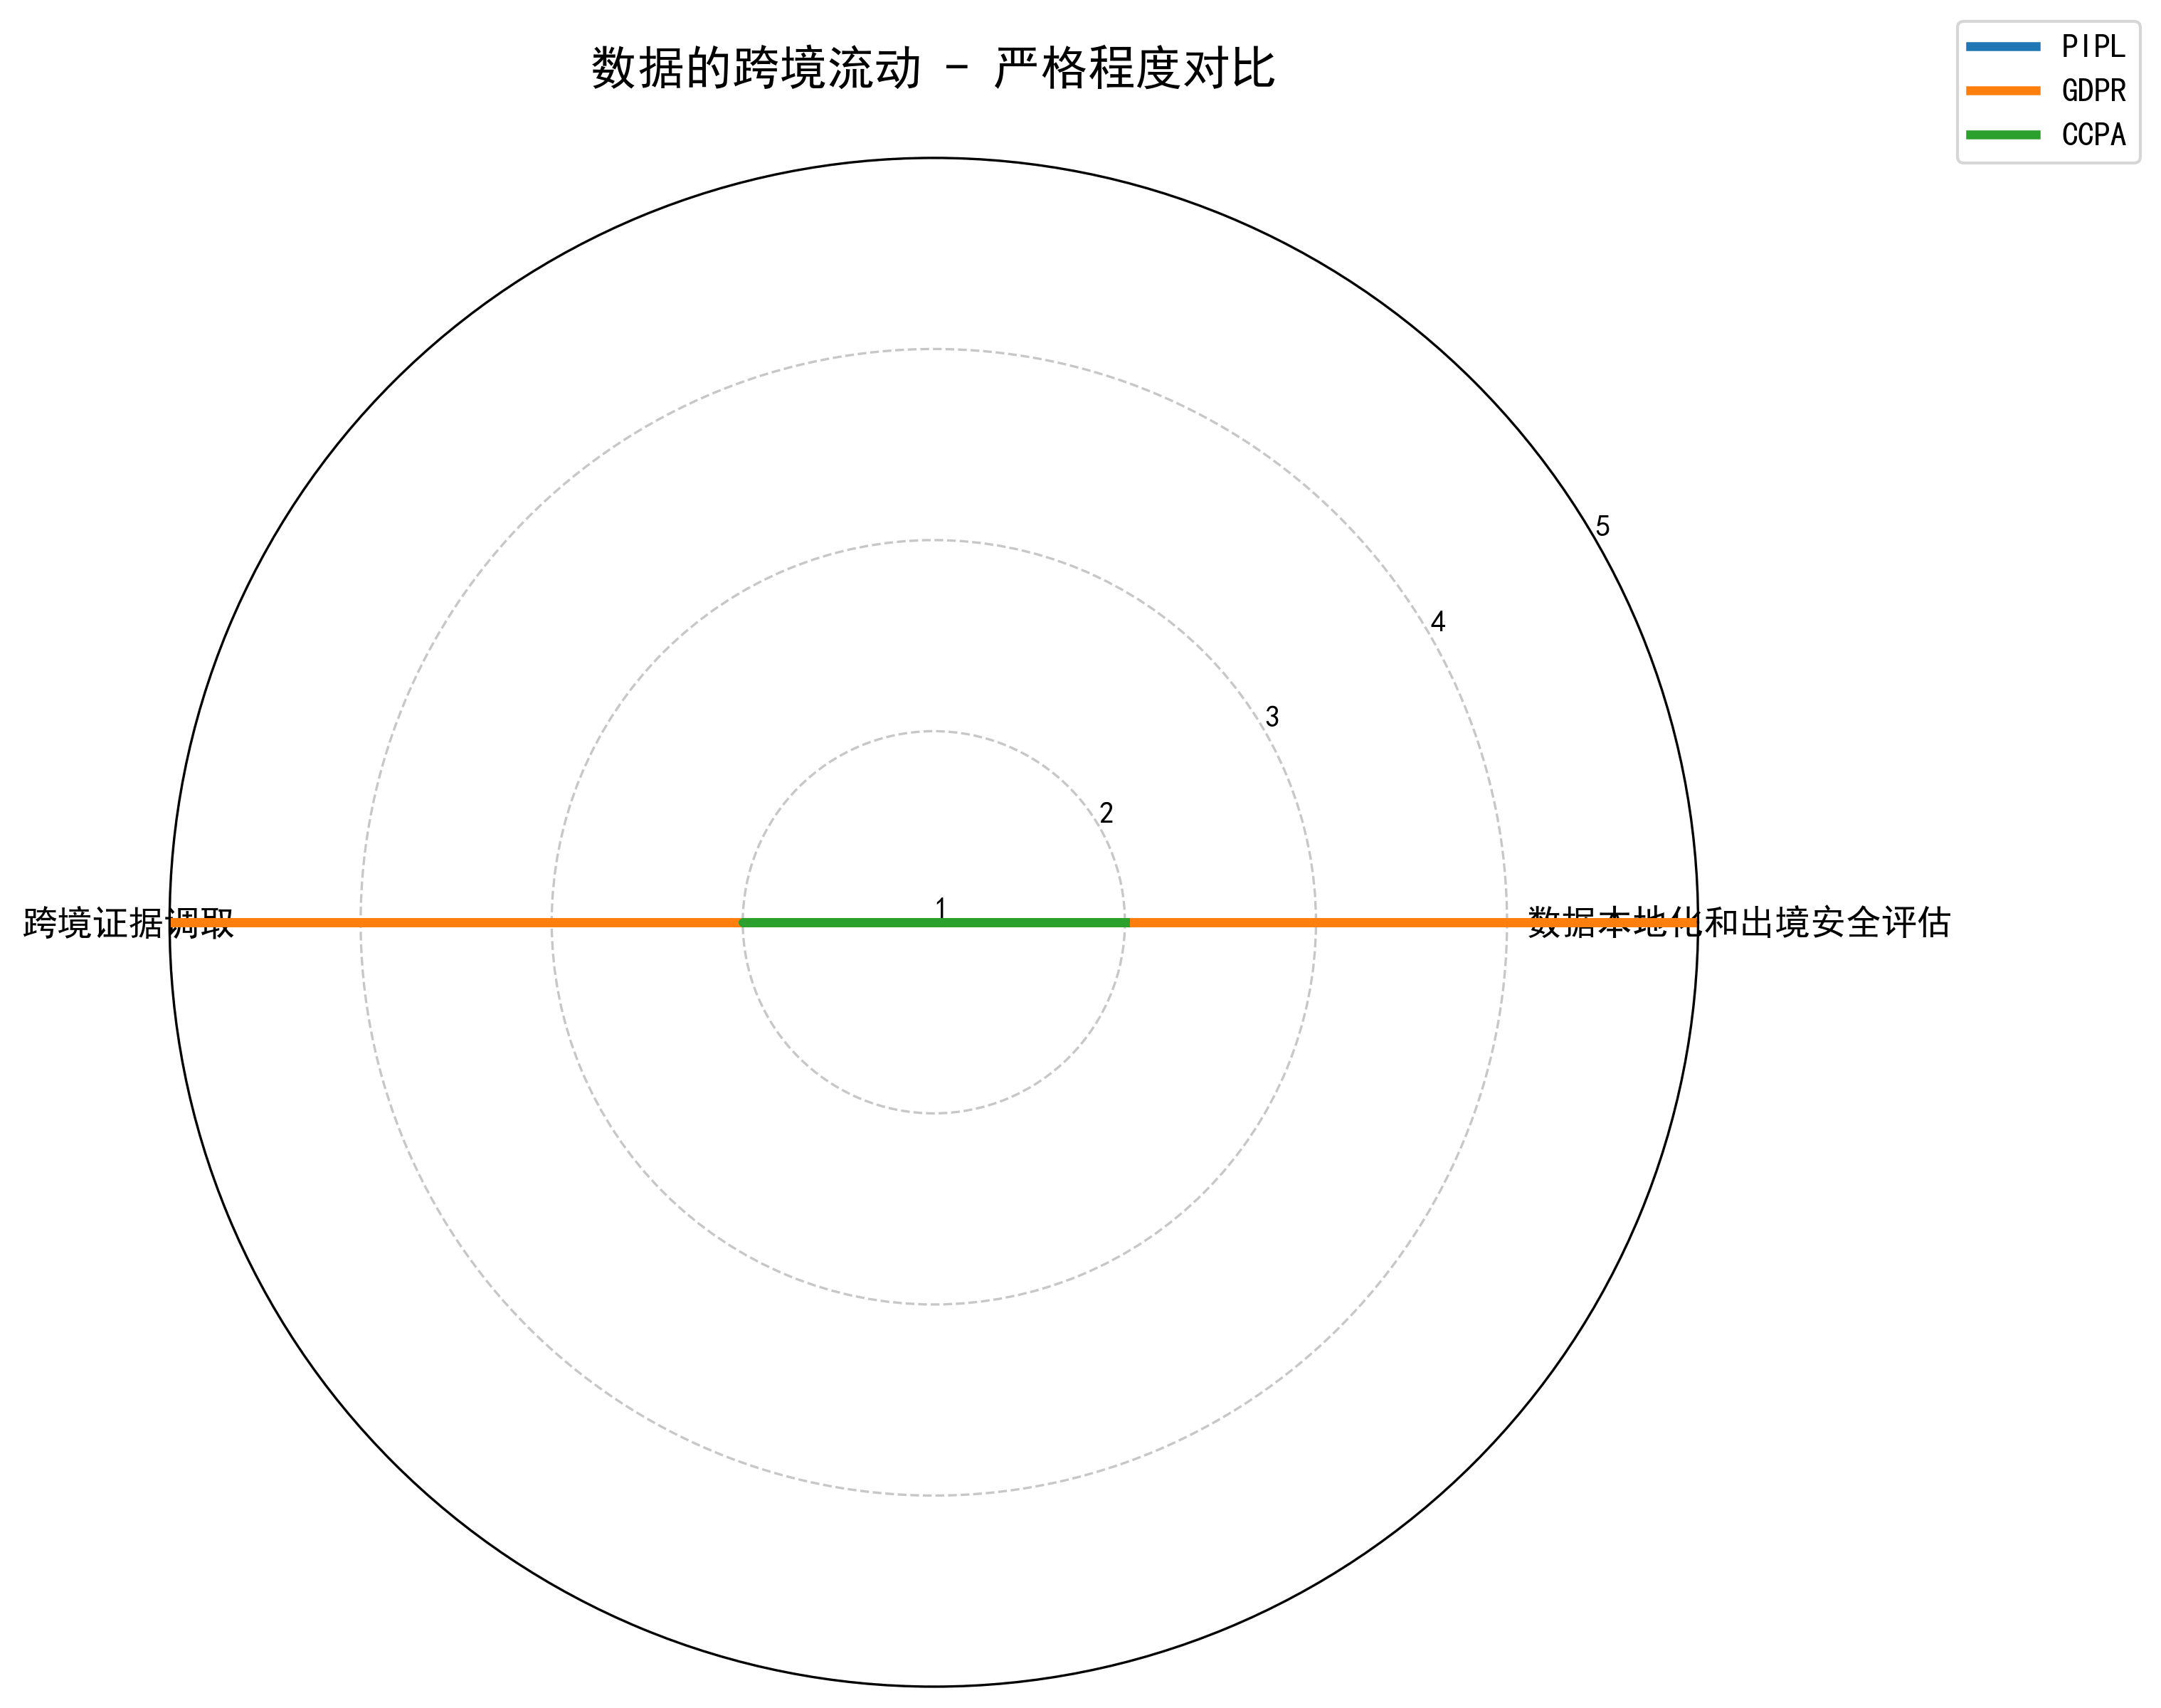
\includegraphics[width=0.8\textwidth]{pics/radar_数据的跨境流动_strictness.png}
	\end{figure}
\end{frame}


\subsection{监管与法律责任}
\begin{frame}
	\frametitle{监管与法律责任}
	\footnotesize
	\begin{tabularx}{\textwidth}{X|X|X|X}
		\toprule
		\textbf{比较点} & \textbf{PIPL} & \textbf{GDPR} & \textbf{CCPA} \\
		\midrule
		监管机构 & 国家网信部门统筹；工信、市监等多部门 & 各国独立监管机构；EDPB协调 & 加州隐私保护局（CPPA）和总检察长（AG） \\
		行政处罚/罚款 & 一般：最高100万；严重：5000万以下或上一年度营业额5\%；对责任人10-100万 & 一般：1000万欧元或2\%；严重：2000万欧元或4\% & CPPA：每项最高2500美元（一般）/7500美元（故意/涉及未成年人）；AG同 \\
		私人诉讼权 & 过错推定原则，赔偿按损失或获利 & 数据主体有权获损害赔偿 & 仅限数据泄露情形（未加密/未编辑），赔偿100-750美元；需30天通知并给纠正机会 \\
		\bottomrule
	\end{tabularx}
\end{frame}

\begin{frame}
	\frametitle{监管与法律责任}
	\footnotesize
	\begin{tabularx}{\textwidth}{X|X|X|X}
		\toprule
		\textbf{比较点} & \textbf{PIPL} & \textbf{GDPR} & \textbf{CCPA} \\
		\midrule
		公益诉讼 & 检察院、消费者组织、网信部门确定的组织可提起 & 非营利组织可代表数据主体 & 无明确规定 \\
		信用记录 & 违法行为记入信用档案并公示 & 无 & 无 \\
		刑事责任 & 构成犯罪的依法追究 & 成员国可规定其他处罚 & 无明确规定 \\
		其他特色 & 反规避条款（无明确）；约谈制度；合规审计 & 合作与一致性机制；紧急程序；互助 & 反规避条款（有）；消费者隐私基金；5年执法时效 \\
		\bottomrule
	\end{tabularx}
\end{frame}

\begin{frame}
	\frametitle{监管与法律责任 - 星级对比}
	\centering
	\textbf{作用范围星级对比}
	\begin{figure}
		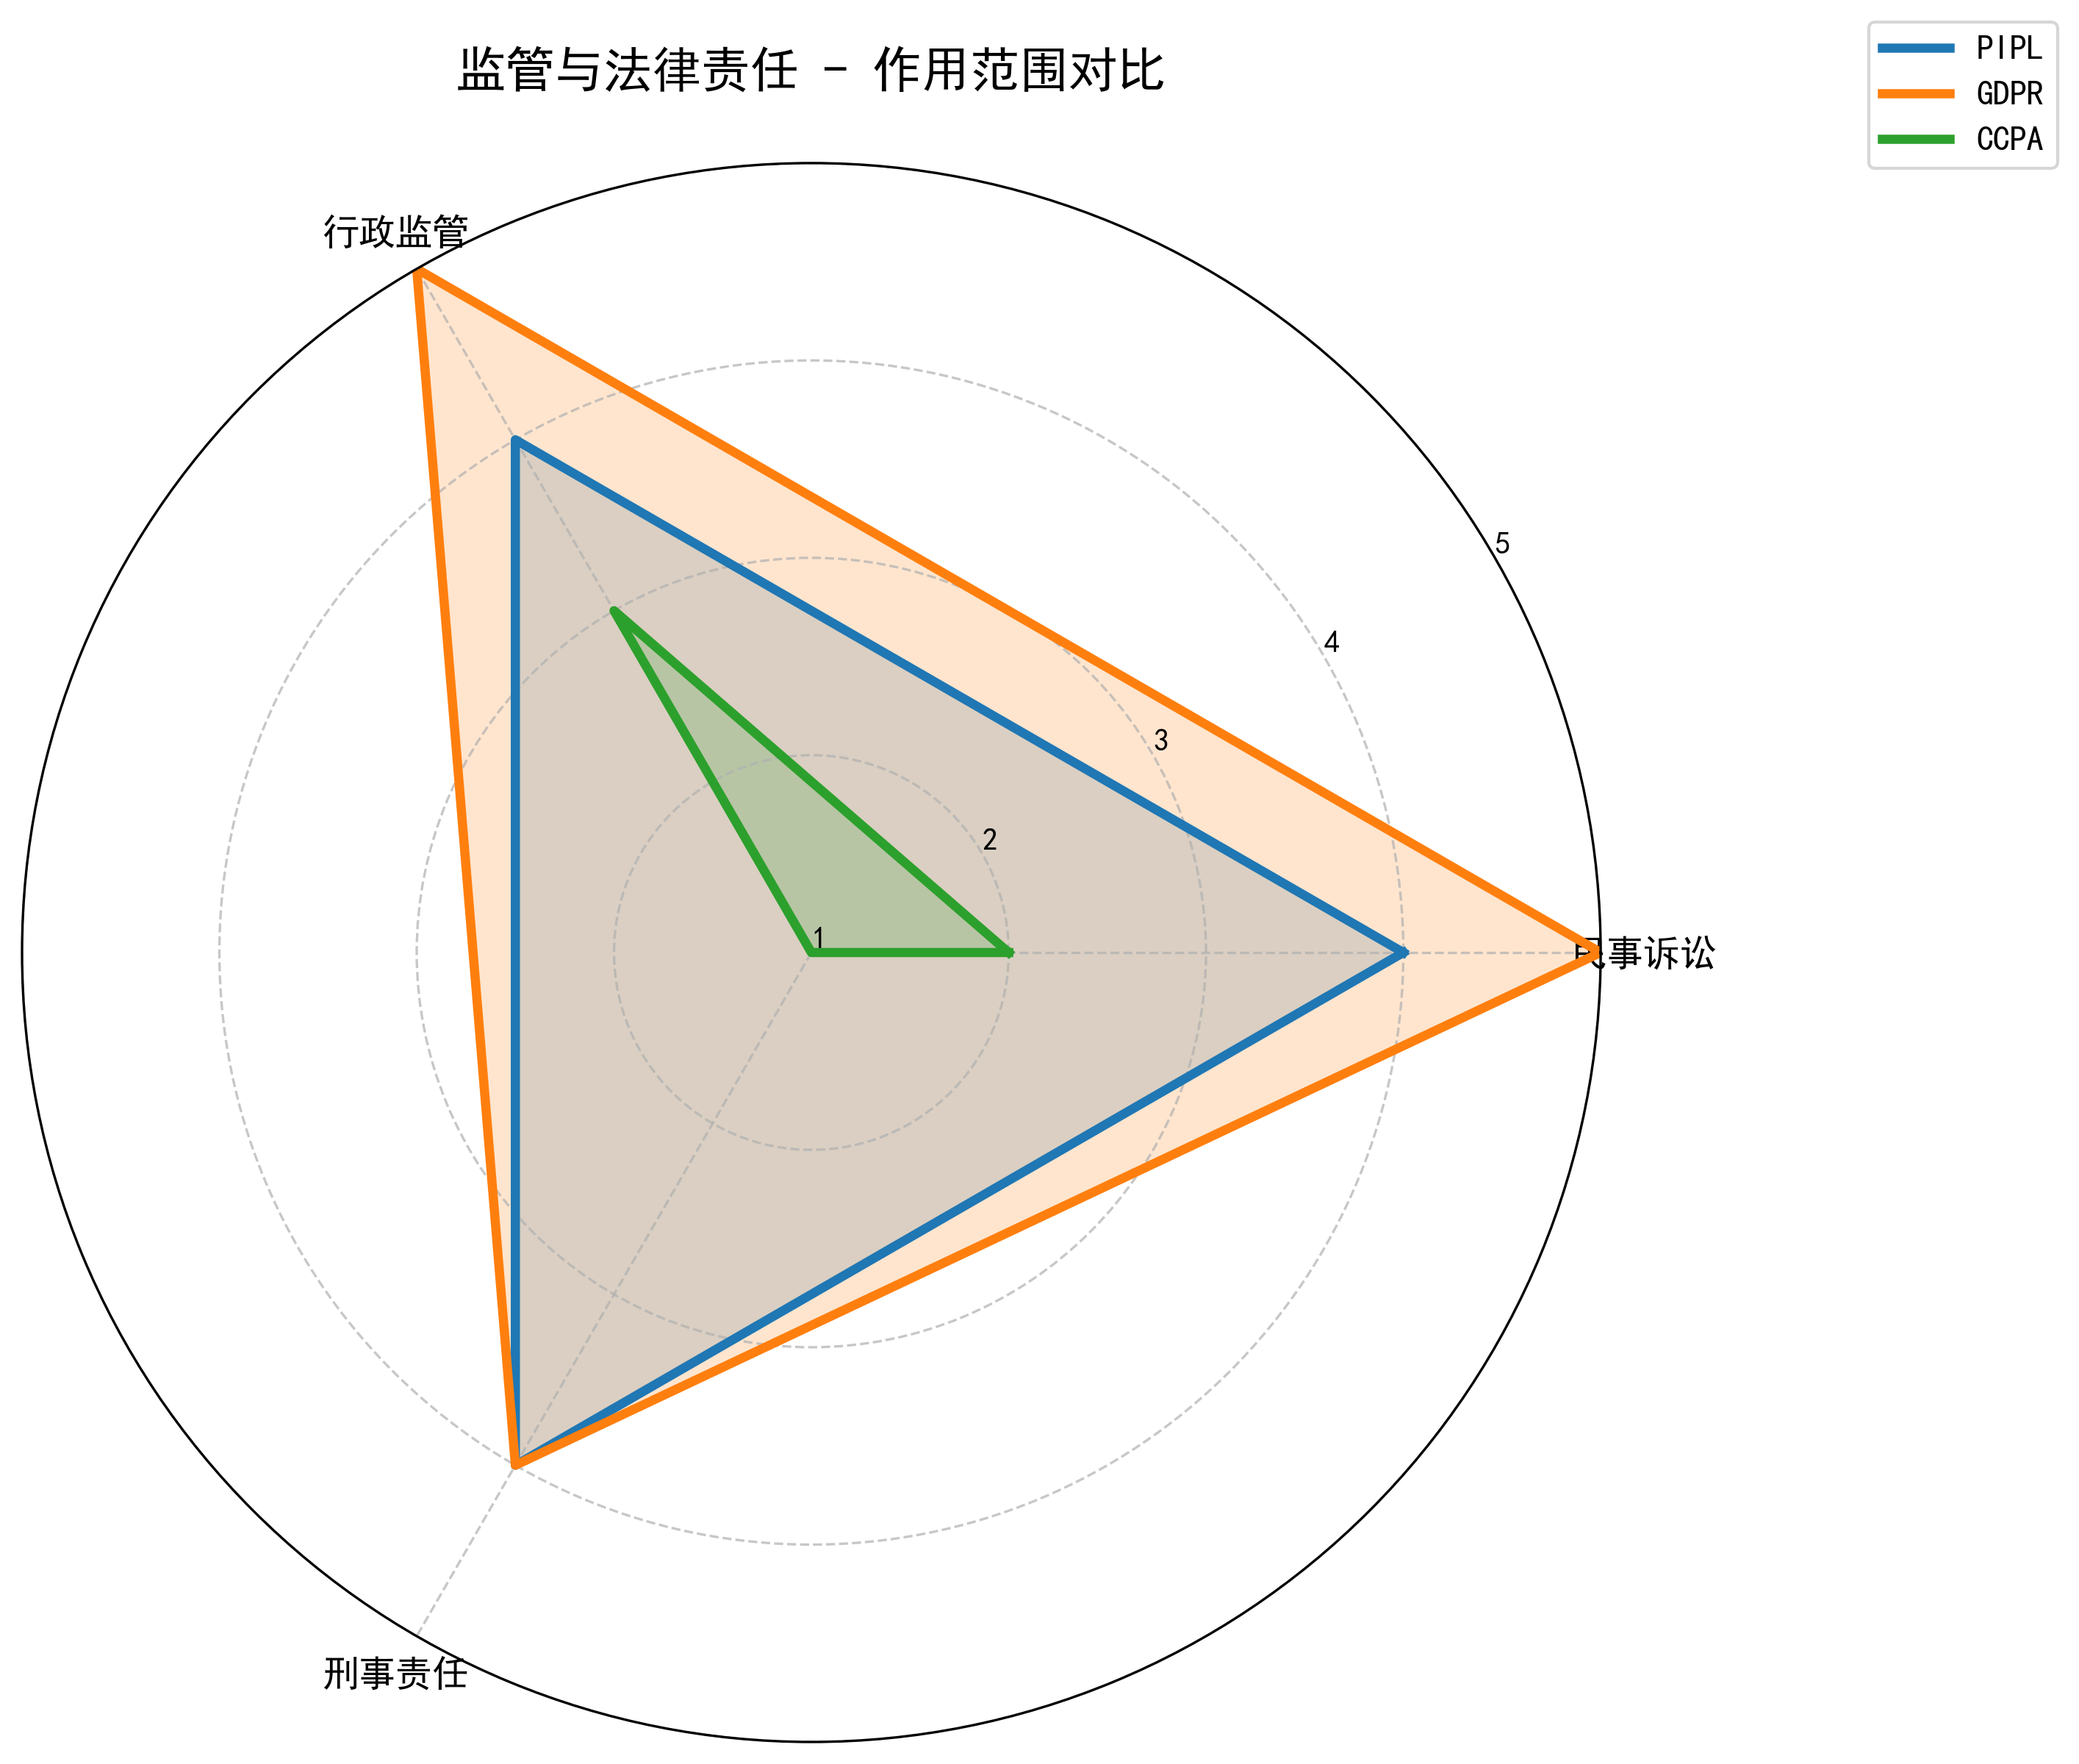
\includegraphics[width=0.8\textwidth]{pics/radar_监管与法律责任_scope.png}
	\end{figure}
	
\end{frame}

\begin{frame}
	\frametitle{监管与法律责任 - 星级对比}
	\centering
	
	\textbf{严格程度星级对比}
	\begin{figure}
		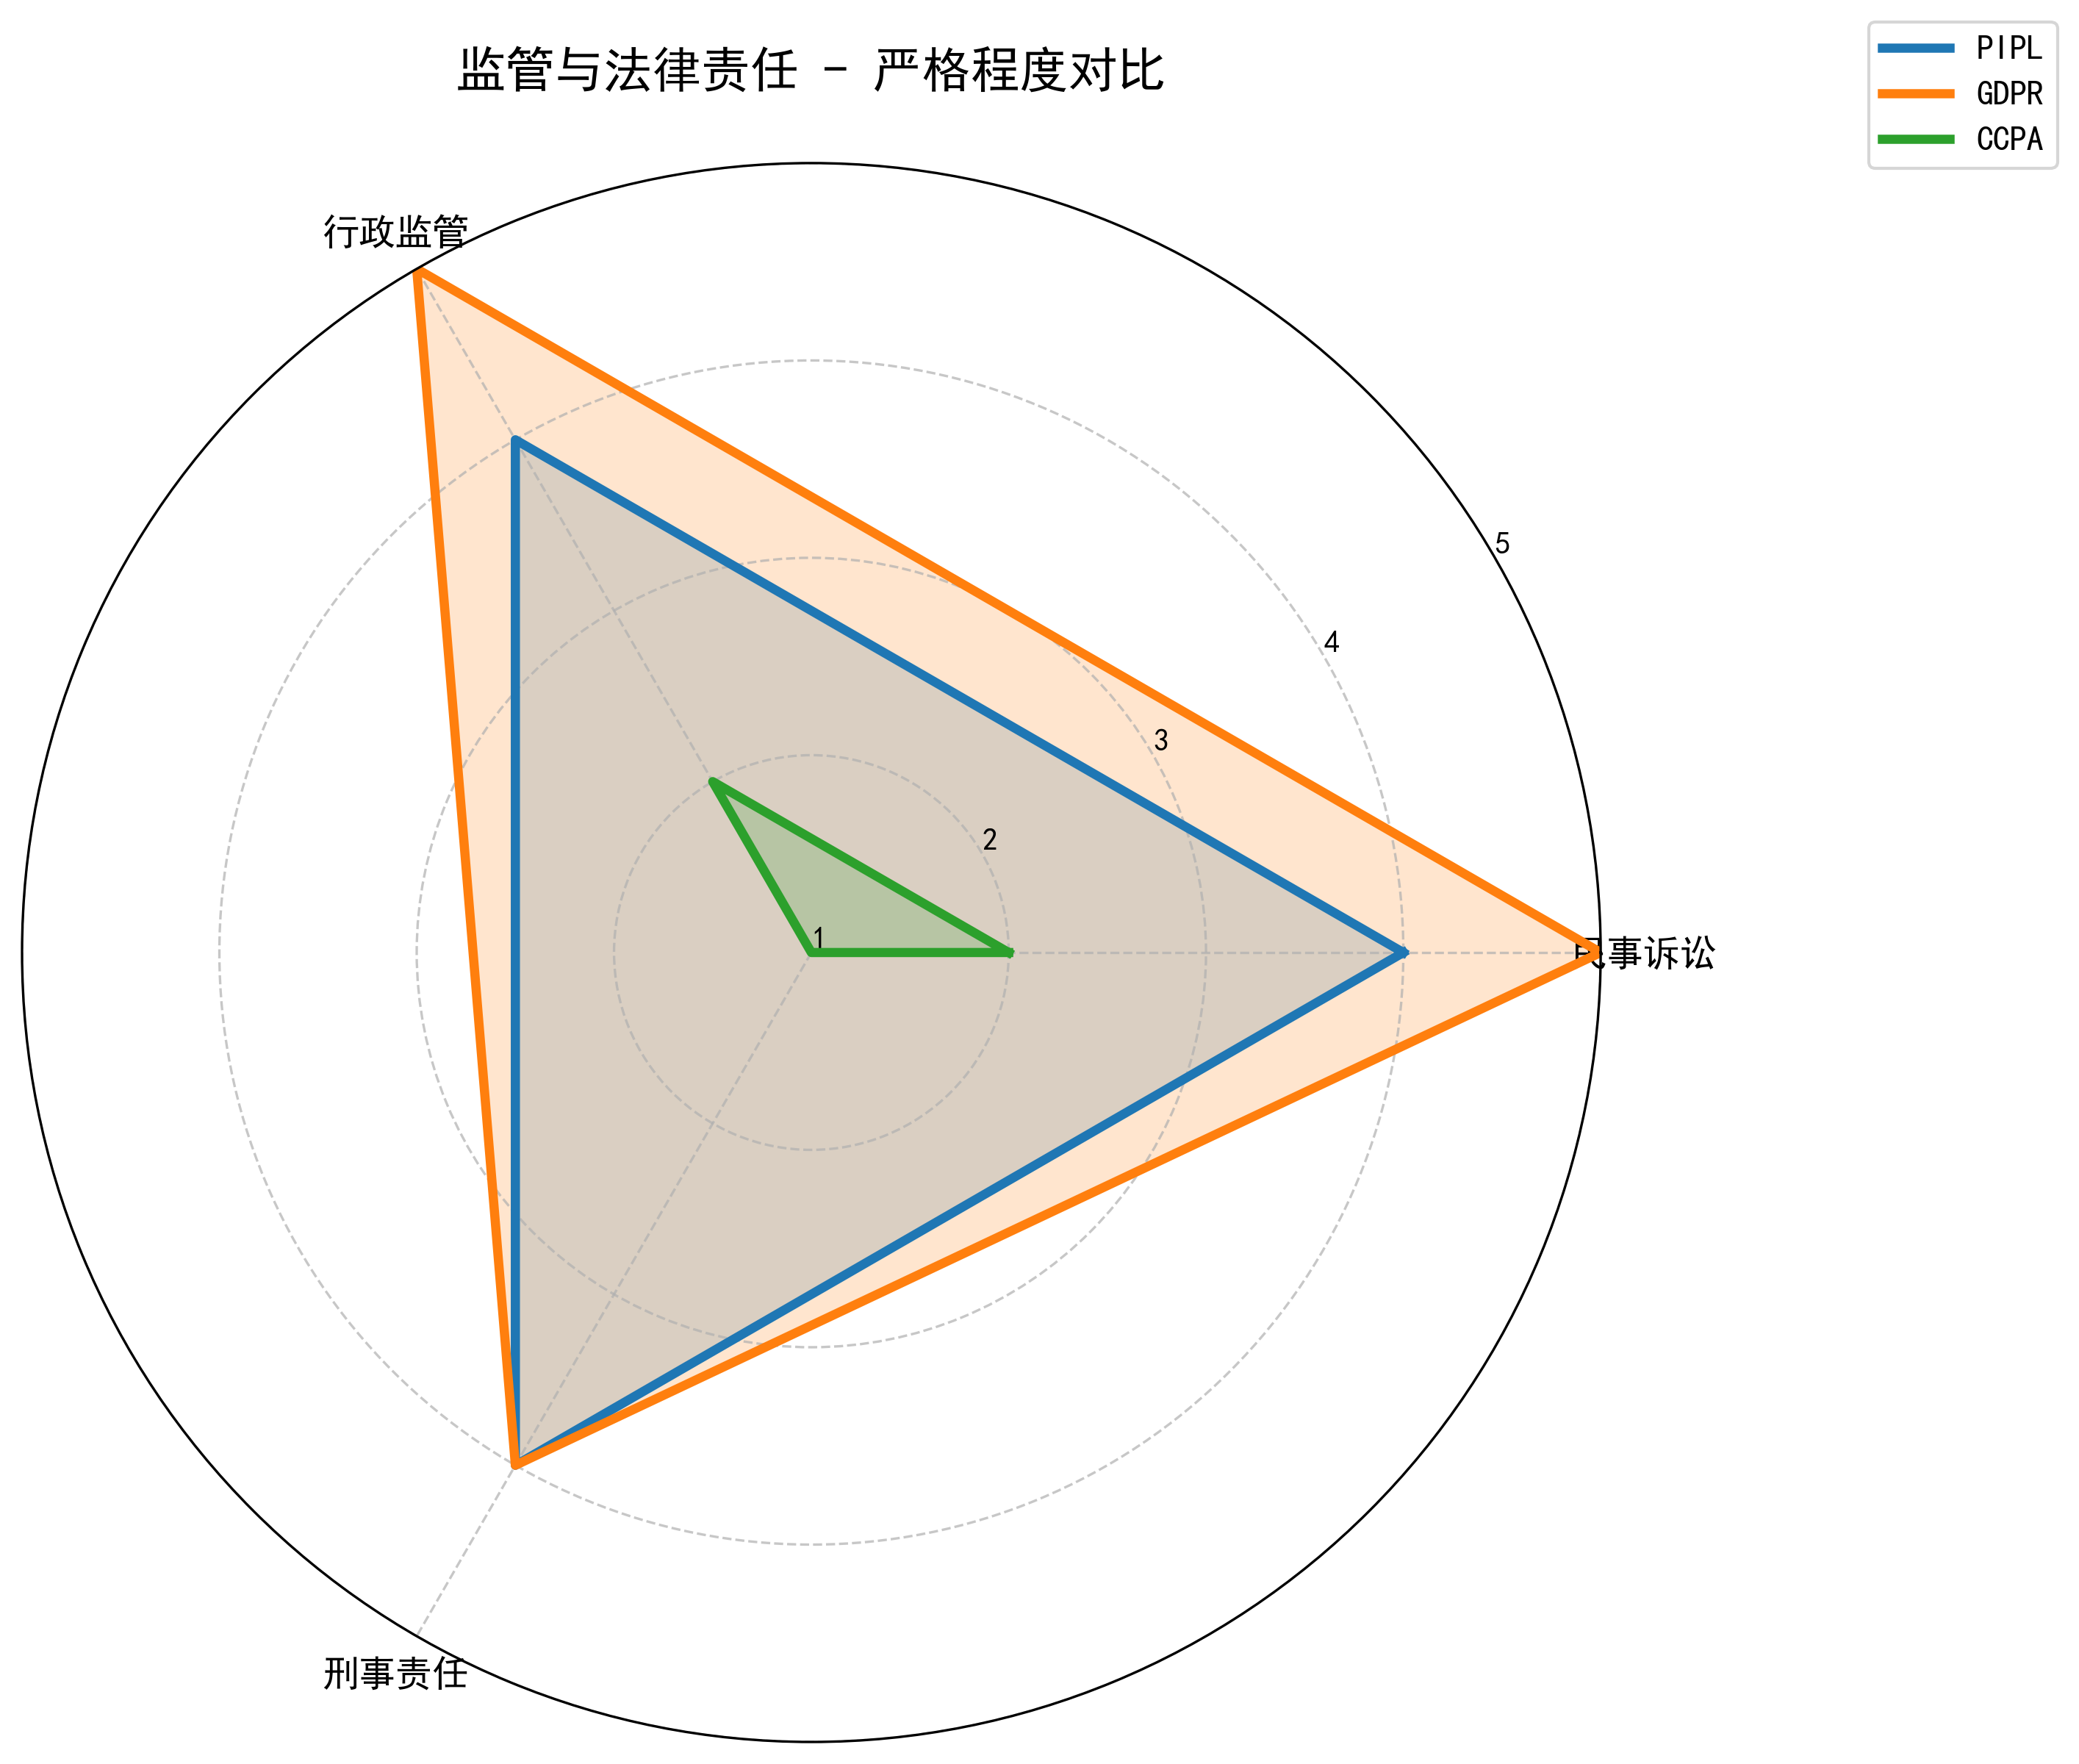
\includegraphics[width=0.8\textwidth]{pics/radar_监管与法律责任_strictness.png}
	\end{figure}
\end{frame}


\subsection{综合对比}
\begin{frame}
	\frametitle{综合对比 - 作用范围}
	\centering
	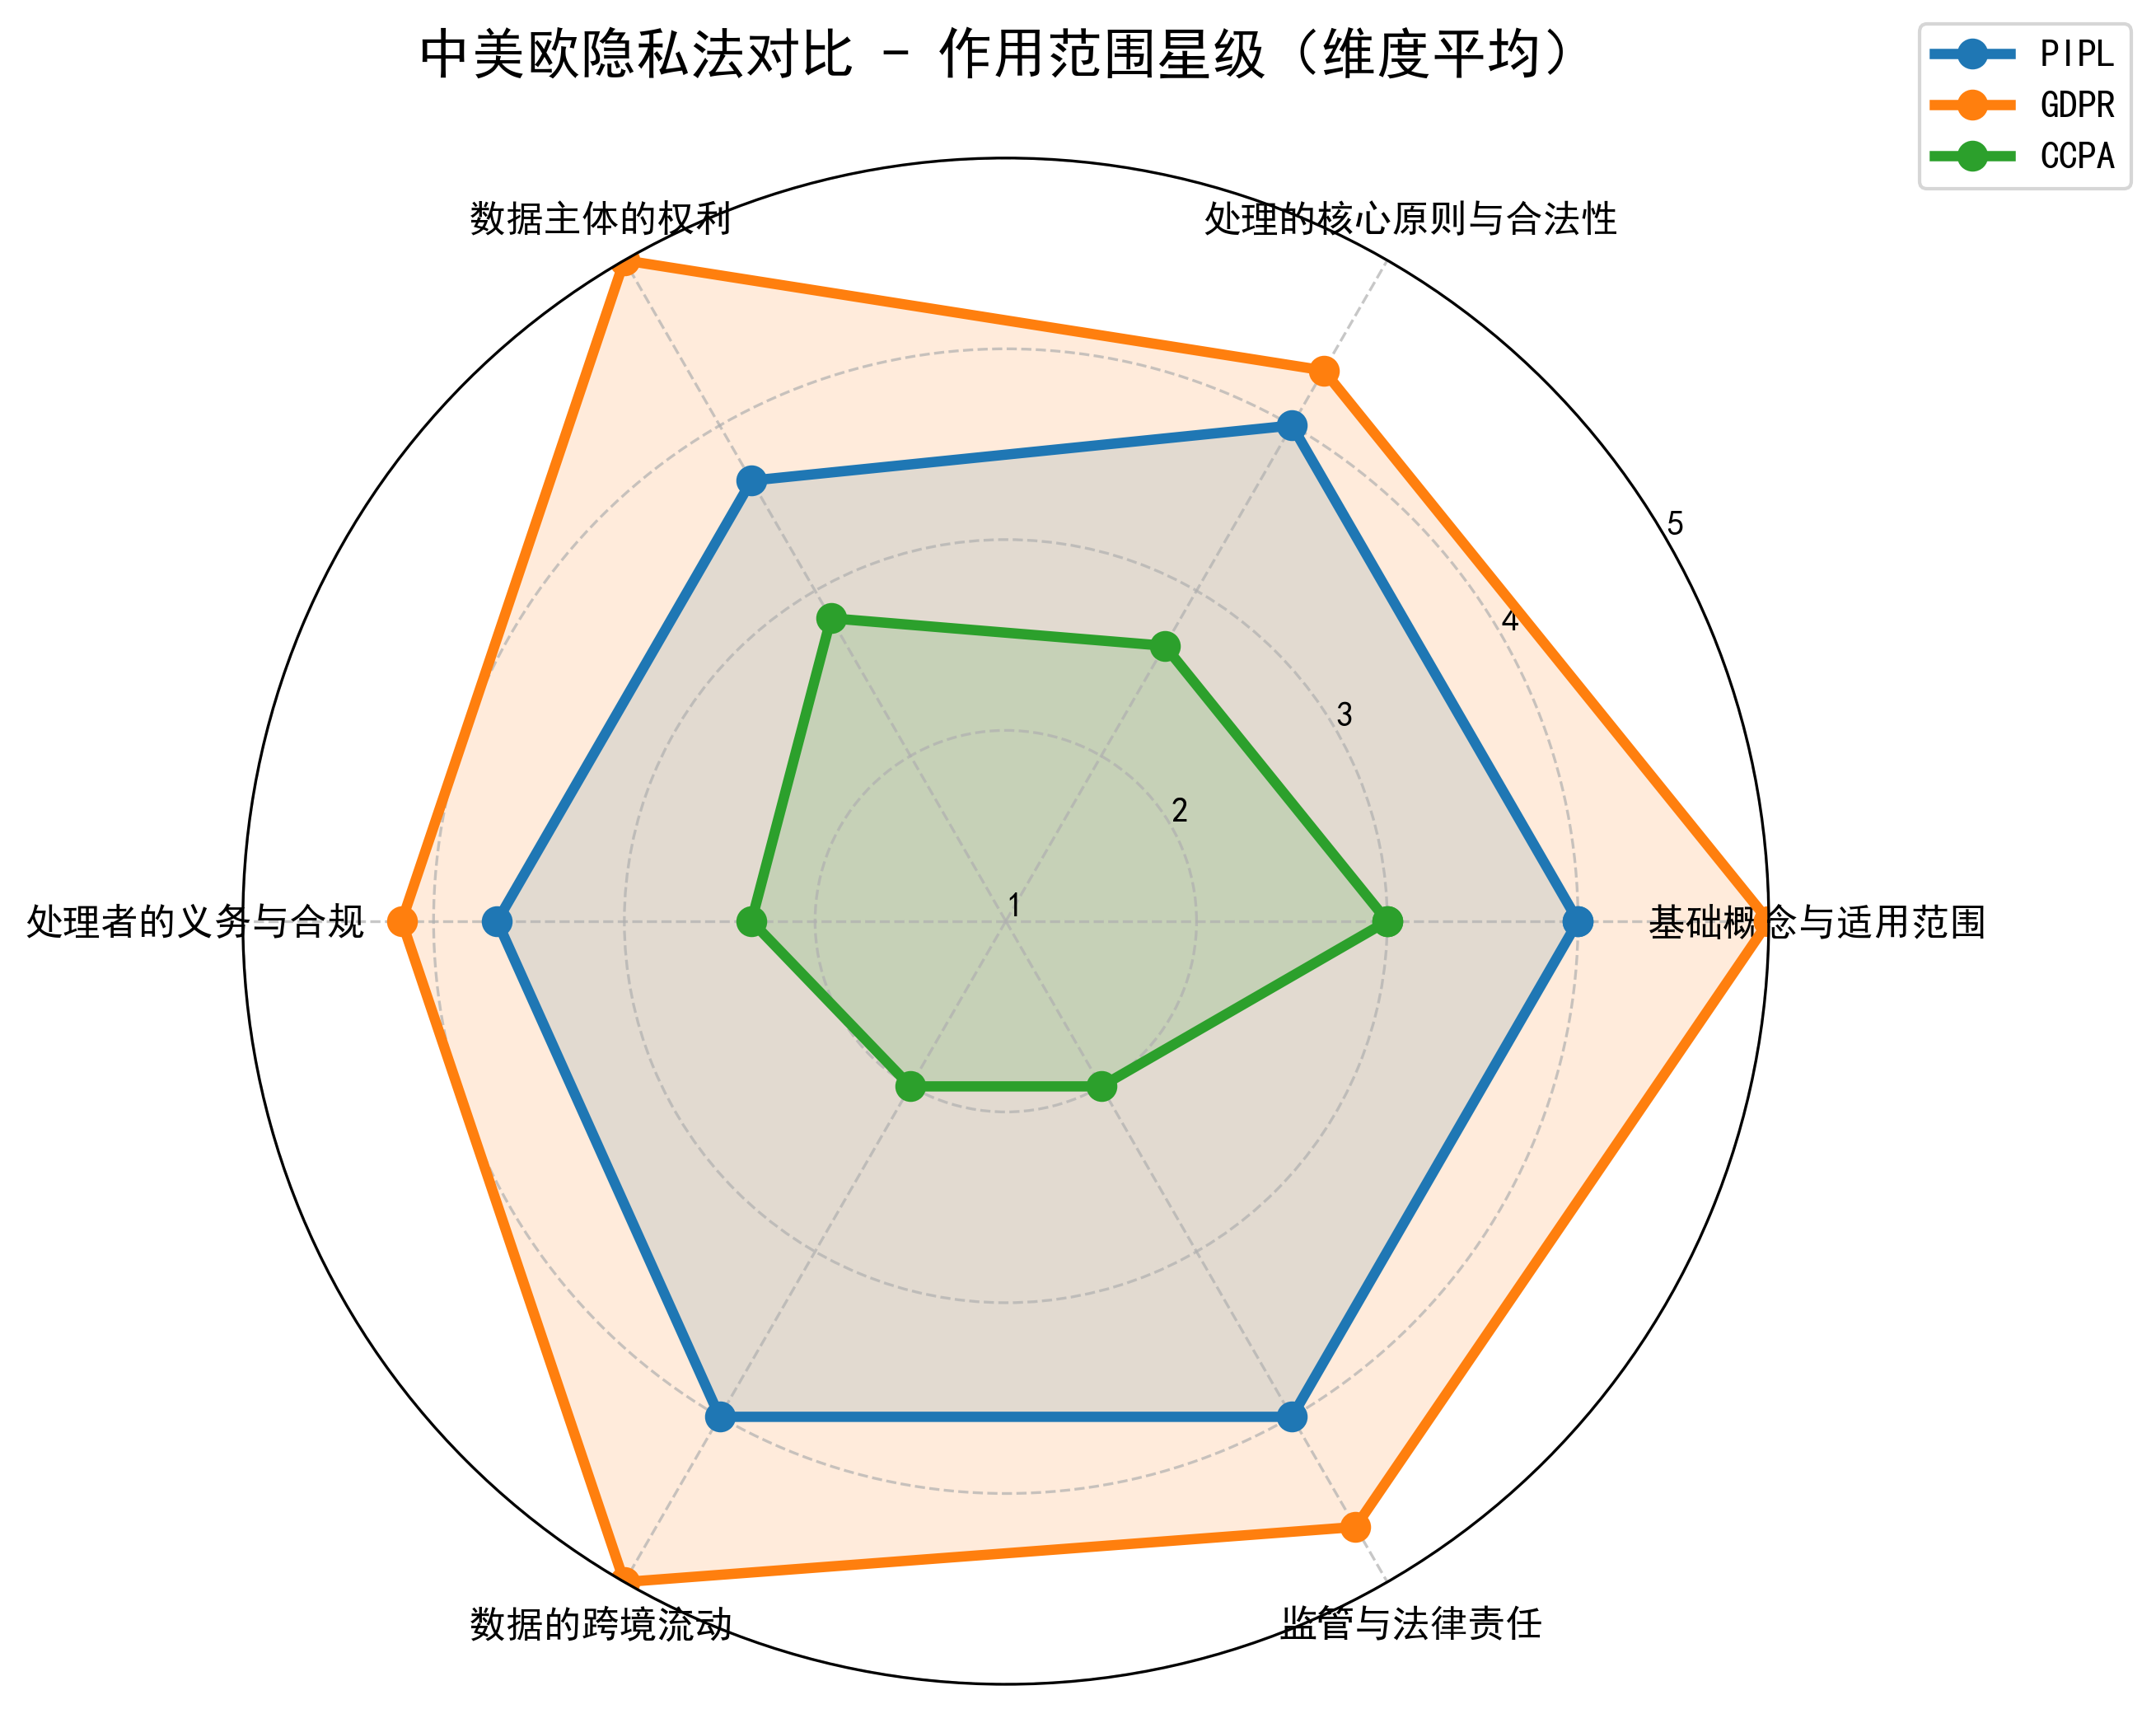
\includegraphics[width=0.85\textwidth]{pics/radar_summary_scope.png}
	
	\textbf{六个维度作用范围平均星级对比}
	
	\vspace{0.5em}
	\footnotesize
	注：雷达图展示了PIPL、GDPR、CCPA在六个维度上的平均作用范围星级评分
\end{frame}

\begin{frame}
	\frametitle{综合对比 - 严格程度}
	\centering
	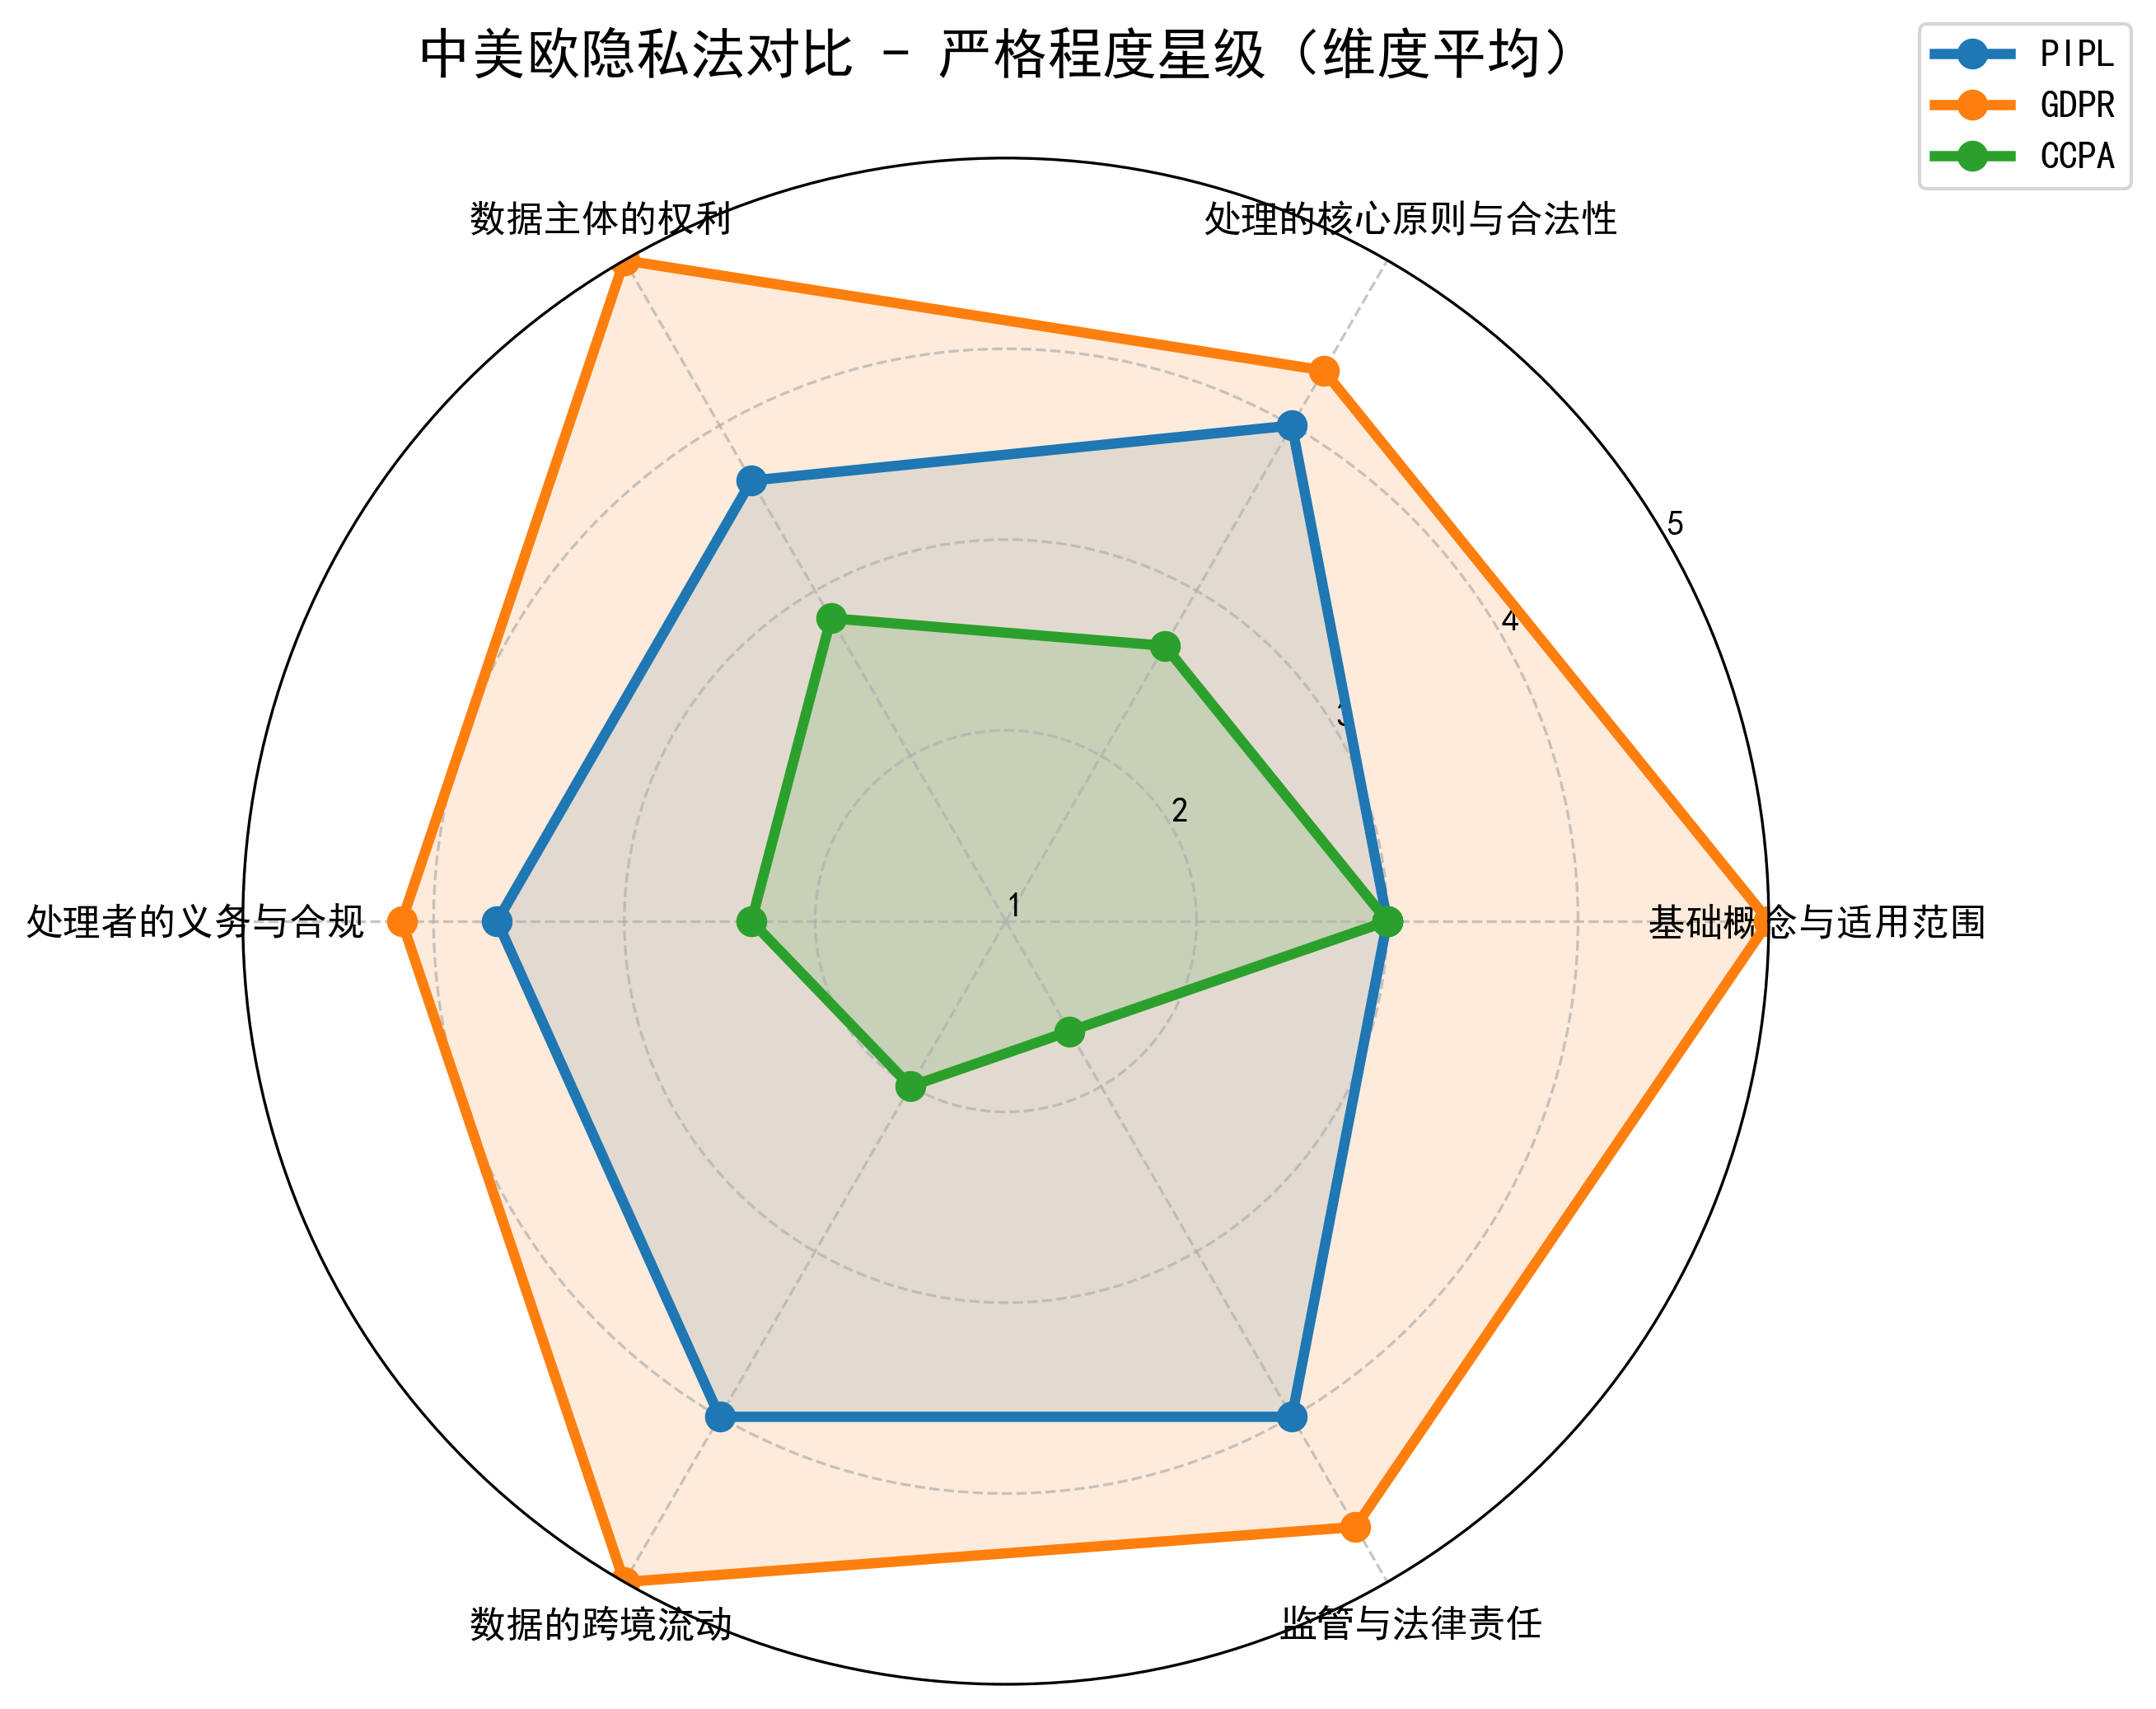
\includegraphics[width=0.85\textwidth]{pics/radar_summary_strictness.png}
	
	\textbf{六个维度严格程度平均星级对比}
	
	\vspace{0.5em}
	\footnotesize
	注：雷达图展示了PIPL、GDPR、CCPA在六个维度上的平均严格程度星级评分
\end{frame}

\section{结论与展望}
\begin{frame}
	\frametitle{结论与展望}
	\begin{itemize}
		\item GDPR在六个维度均保持最严格标准和最广适用范围，是隐私保护的标杆。
		\item PIPL在大型平台义务、敏感信息保护、境内存储等方面有独特强化，但部分细则尚未落地。
		\item CCPA通过CPRA修订（2026年新规）正向欧盟标准靠拢，但整体仍较为宽松。
		\item 基于以上对比，隐私检测软件可针对不同法域动态配置合规规则：
		\begin{itemize}
			\item 跨境流动：评估传输机制是否满足安全评估、SCC或合同要求。
			\item 法律责任：根据违规类型预估罚款风险及私人诉讼触发条件。
			\item 主体权利：提供知情、访问、删除、选择退出等自动化响应接口。
		\end{itemize}
	\end{itemize}
\end{frame}

\begin{frame}
	\begin{center}
		{\Huge 感谢聆听！}
	\end{center}
\end{frame}

\end{document}
